\documentclass[11pt]{article}
\usepackage{times}
\usepackage{verbatim}
\usepackage[pdftex]{graphicx}    
\usepackage[pdftex]{color}  
\usepackage{fullpage}
\usepackage{url}
\usepackage{cite}

\bibliographystyle{plos}

% \draftfalse: submission version. Legends,tables at end. No figs included.
% \drafttrue:   online preprint. Figures and table inline.
\newif\ifdraft
%\draftfalse
\drafttrue

\renewcommand{\baselinestretch}{1.5}
\setcounter{secnumdepth}{0}


\begin{document}

\title{Query-Dependent Banding (QDB) for Faster RNA Similarity Searches}
\author{Eric P. Nawrocki and Sean R. Eddy\\
HHMI Janelia Farm Research Campus\\
19700 Helix Drive\\
Ashburn VA 20147\\
\url{http://selab.janelia.org/}\\
}
%\date{\today}
\maketitle

\begin{center}
\textbf{Running head:} Faster RNA Similarity Searches
\end{center}



%%%%%%%%%%%%%%%%%%%%%%%%%%%%%%%%%%%%%%%%%%%%%%%%%%%%%%%%%%%%%%%%%%%%%%

\begin{abstract}

When searching sequence databases for RNAs, it is desirable to score
both primary sequence and RNA secondary structure similarity.
Covariance models (CMs) are probabilistic models well suited for RNA
similarity search applications. However, the computational complexity
of CM dynamic programming alignment algorithms has limited their
practical application. Here we describe an acceleration method called
\emph{query-dependent banding} (QDB), which uses the probabilistic
query CM to precalculate regions of the dynamic programming lattice
that have negligible probability, independently of the target
database. We have implemented QDB in the freely available
\textsc{infernal} software package. QDB reduces the average-case time
complexity of CM alignment from $LN^{2.4}$ to $LN^{1.3}$ for a query
RNA of $N$ residues and a target database of $L$ residues, resulting
in a four-fold speedup for typical RNA queries. Combined with other
improvements to \textsc{infernal}, including informative mixture
Dirichlet priors on model parameters, benchmarks also show increased
sensitivity and specificity resulting from improved parameterization.

\end{abstract}


%%%%%%%%%%%%%%%%%%%%%%%%%%%%%%%%%%%%%%%%%%%%%%%%%%%%%%%%%%%%%%%%%%%%%%

\section{Introduction}

Many functional RNAs conserve a base-paired secondary structure.
Conserved RNA secondary structure induces long-distance pairwise
correlations in homologous RNA sequences.  When performing database
searches to identify homologous structural RNAs, it is desirable for
RNA similarity search programs to score a combination of secondary
structure and primary sequence conservation.

A variety of approaches for RNA similarity searching have been
described. There are specialized programs for identifying one
particular RNA family or motif, such as programs that identify tRNAs
\cite{LoweEddy97,Laslett04}, snoRNAs \cite{LoweEddy99,Schattner06},
microRNAs \cite{Lai03, Lim03}, SRP RNAs \cite{Regalia02}, and
rho-independent transcription terminators \cite{Ermolaeva00}. There
are also pattern-matching algorithms that rely on expertly designed
query patterns \cite{Macke01}. However, the most generally useful
approaches are those that take any RNA (or any multiple RNA alignment)
as a query, and use an appropriate scoring system to search a sequence
database and rank high-scoring similarities
\cite{Gautheret01,ZhangBafna05}, just as programs like \textsc{blast}
do for linear sequence comparison \cite{Altschul97}.

In a general search program, one wants to score a
combination of RNA sequence and structural conservation in a
principled rather than \emph{ad hoc} manner. A satisfactory solution
to this problem is known, using probabilistic models called
\emph{stochastic context-free grammars} (SCFGs). SCFGs readily capture
both primary sequence and (non-pseudoknotted) RNA secondary structure
conservation \cite{Sakakibara94c,Durbin98}. Just as hidden Markov
models (HMMs) are useful for many different linear sequence modeling
applications, including genefinding, multiple alignment, motif
finding, and similarity search \cite{Durbin98}, SCFGs are a generally
useful paradigm for probabilistic RNA sequence/structure analysis,
with applications including secondary structure prediction and
genefinding. A particular SCFG architecture called \emph{covariance
models} (CMs) was developed specifically for the RNA similarity search
problem \cite{Eddy94}.  CMs are profile SCFGs, analogous to the use of
profile HMMs in sequence analysis \cite{Eddy94,Eddy02b}.  The Rfam
database of RNA families \cite{Griffiths-Jones05} is based on CM
software (\textsc{infernal}) in much the same way that the Pfam
database of protein families is based on profile HMM software
(\textsc{hmmer}) \cite{Sonnhammer98,Finn06}.

The most serious problem with using CMs has been their computational
complexity. Applying standard SCFG dynamic programming alignment
algorithms to the particular case of CMs results in algorithms that
require $O(N^3)$ memory and $O(L N^3)$ time for a query of length $N$
residues (or consensus alignment columns) and a target database
sequence of length $L$.  The memory complexity problem has essentially
been solved, by extending divide-and-conquer dynamic programming
methods (the Hirshberg or Myers/Miller algorithm) to the case of CMs
\cite{Eddy02b}, but the time complexity problem still stands.

Weinberg and Ruzzo have described several filtering methods for
accelerating CM searches
\cite{WeinbergRuzzo04,WeinbergRuzzo04b,WeinbergRuzzo06}. The original
idea (``rigorous filters'') was to score a target sequence first by a
linear sequence comparison method, using a profile HMM specially
constructed from the query CM such that the profile score was provably
an upper bound on the CM score; the subset of hits above threshold
would then be passed for rescoring with the more expensive CM
alignment algorithm \cite{WeinbergRuzzo04b}.  Subsequently a ``maximum
likelihood heuristic'' filter profile was developed that gives up the
guarantee of recovering the same hits as the unfiltered search, but
offers greater speedups \cite{WeinbergRuzzo06}.  For most current Rfam
models, Weinberg/Ruzzo filters give about a hundred-fold speed up
relative to a full CM based search at little or no cost to sensitivity
and specificity. However, because these filters depend on primary
sequence conservation alone, they can be relatively ineffective for
RNA families that exhibit poor sequence conservation -- unfortunately,
precisely the RNAs that benefit the most from SCFG-based search
methods.  Indeed, in this respect, we are concerned that the overall
performance of rigorous filters on the current Rfam database may be
somewhat misleading. Rfam currently uses a crude \textsc{blast}-based
filtering method to accelerate the CM searches used in curating the
database. This step introduces a bias towards high primary sequence
similarity in current Rfam alignments. As Rfam improves and
incorporates more diverse structural homologs, the effectiveness of
sequence-based filters will decrease. To address this worry, Weinberg
and Ruzzo have also described additional heuristics (``sub-CMs'' and
the ``store-pair'' technique) that should capture more secondary
structure information in the filtering process
\cite{WeinbergRuzzo04}. Bafna and coworkers have described further
improvements to sequence filtering methods \cite{ZhangBafna06}.
Currently, the \textsc{infernal} codebase includes Weinberg's C++
implementation of rigorous filters, but not, as yet, the ML heuristic,
sub-CM, or store-pair methods.  All these methods are important, but
it also remains important to us to identify yet more methods for
accelerating CMs.

Here, we describe a method for accelerating CM searches using a banded
dynamic programming (DP) strategy. In banded DP, one uses some fast
method to identify a band through the DP matrix where the optimal
alignment is likely to lie, and then calculates computationally
expensive DP recursions only within that band. In most cases,
including our approach, banded DP is a heuristic that sacrifices
guaranteed alignment optimality. Banding is a standard approach in
many areas of sequence analysis. Gapped \textsc{blast} uses banded DP
to convert ungapped high-scoring pairs (HSPs) to full gapped
alignments \cite{Altschul97}.  \textsc{lagan} and \textsc{multi-lagan}
use banded dynamic programming (referred to as limited-area dynamic
programming) to stitch together alignments between anchored sequences
when aligning long genomic sequences \cite{Brudno03}. Banding has also been
applied to profile SCFGs by Michael Brown in his \textsc{rnacad}
program by using information from a profile HMM alignment to define
bands for the expensive SCFG alignment \cite{Brown00}. The key to
developing a banded DP strategy is in deciding how the bands are
identified.  Usually, including all the examples just mentioned,
banded DP involves performing some sort of rapid approximate sequence
alignment between the query and the target.

In contrast, the method we describe here, called \emph{query-dependent
banding} (QDB), takes advantage of specific properties of CMs in order
to predefine bands that are independent of any target sequence.  QDB
depends on the consensus secondary structure of the query, so it is
complementary to acceleration methods like the Weinberg/Ruzzo filters
that rely on sequence but not structure.



\section{Results}

Briefly, the key idea is the following. Each base pair and each
single-stranded residue in the query RNA is represented in a CM by a
\emph{state}. States are arranged in a tree-like structure that
mirrors the secondary structure of the RNA, along with additional
states to model insertions and deletions. The standard CM dynamic
programming alignment algorithm works by calculating the probability
that a substructure of the query rooted at state $v$ aligns to a
subsequence $i..j$ in the the target sequence. The calculation is
recursive, starting at the leaves of the CM (ends of hairpin loops)
and subsequences of length 0, and working upwards in larger
substructures of the CM, and outwards in longer and longer
subsequences.

To guarantee optimality, at each $v$, the DP algorithm must score all
possible $i..j$ subsequences in the target sequence.  However, most of
these subsequences are obviously too long or short, when one considers
the size of the query substructure under state $v$.  For example, when
state $v$ models the closing base pair of a consensus four-base loop,
only $i..j$ subsequences of length six are likely to occur in any
optimal alignment to state $v$; that is, $(j-5,j)$ being the base
pair, and $(j-4..j-1)$ being the four bases of the hairpin
loop. Likewise, the optimal subsequence aligned to the next consensus
base pair in that stem is almost certainly of length eight.

Because insertions and deletions may occur in the target sequence, no
subsequence length is known with certainty, but because the CM is a
probabilistic model, a probability distribution for subsequence
lengths under each state (including the probability of insertions and
deletions) can be analytically derived from the query CM.  These
distributions can be used to determine a band of subsequence lengths
that captures all but a negligible amount of the probability mass. A
CM dynamic programming algorithm can then look not at all subsequences
$i,j$ for each state $v$, but only those $i$ within a band of minimum
and maximum distance relative to each $j$.

To formalize this idea, we start with a description of CMs, followed
by the QDB algorithms for calculating the subsequence length
distributions, using these length distributions to determine bands,
and using the bands in a banded CM dynamic programming alignment
algorithm. Calculation of the bands is sensitive to transition
parameter estimation, so we describe \textsc{infernal}'s new
implementation of informative Dirichlet priors for CM parameter
estimation. Finally, we present results from a benchmark that suggest
the sensitivity and specificity of a QDB-accelerated search is
negligibly different from a non-banded search.

\subsection{Covariance models}

CMs are a convention for mapping an RNA secondary structure into a
tree-like, directed graph of SCFG states and state transitions (or
equivalently, SCFG nonterminals and production rules). The CM is
organized by a binary tree of \emph{nodes} representing base pairs and
single-stranded residues in the query's structure.  Each node contains
a number of \emph{states}, where one state represents the consensus
alignment to the query, and the others represent insertions and
deletions relative to the query.  Figure~\ref{fig:cmintro} shows an
example of converting a consensus structure to the guide tree of
nodes, and part of the expansion of those guide tree nodes into the
CM's state graph. Here we will only concentrate on the aspects of CMs
necessary to understand QDB, and a subset of our usual notation. For
full details on CM construction, see \cite{Eddy02b,infguide03}.

\ifdraft
\begin{figure}
\begin{center}
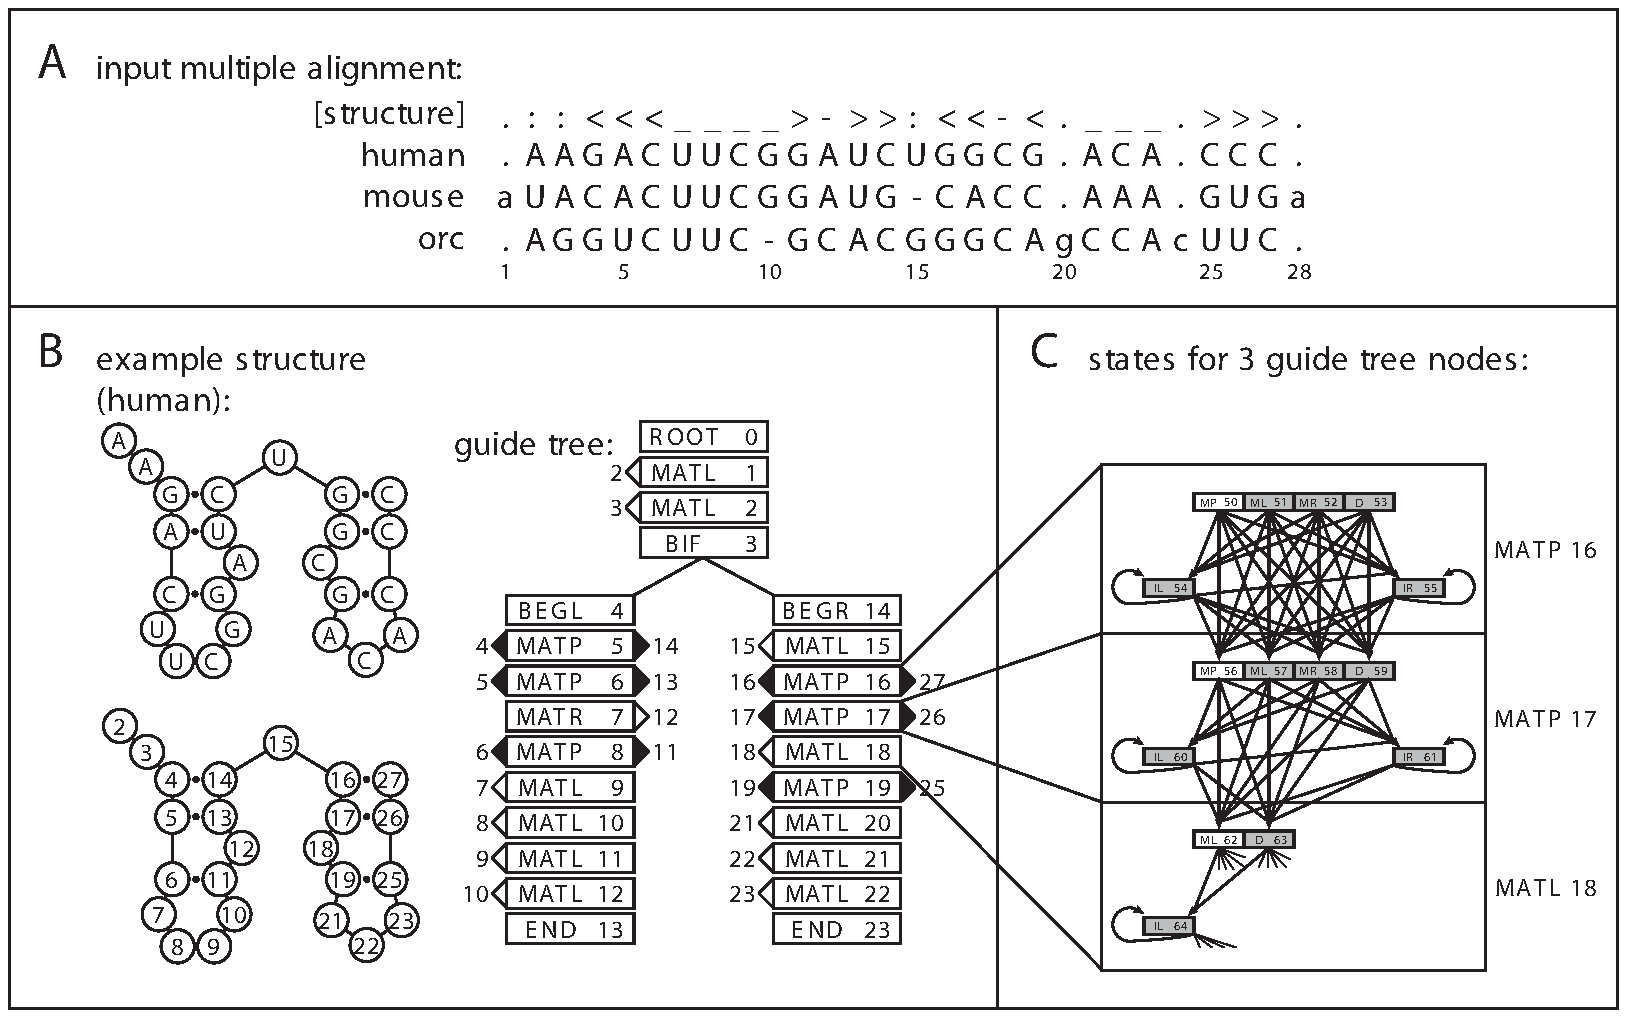
\includegraphics[width=6.4in]{figs/cmintro_bandcyk}
\caption{\textbf{An example RNA family and corresponding CM.}
  \textbf{(A):} A toy multiple alignment of three RNA
  sequences. \textbf{(B):} The structure of one sequence from (A), the
  same structure with positions numbered according to alignment
  columns, and the guide tree of nodes corresponding to that
  structure, with alignment column indices assigned to nodes (for
  example, node 5, a MATP ``match-pair'' node, will model the
  consensus base pair between columns 4 and 14). \textbf{(C):} The
  state topology of three selected nodes of the CM, for two MATP nodes
  and one consensus ``leftwise'' single residue bulge node (MATL,
  ``match-left'').  The consensus pair and singlet states (two MPs and
  one ML) are white, and the insertion/deletion states are grey. State
  transitions are indicated by arrows.}
\label{fig:cmintro}
\end{center}
\end{figure}

% This is \ref{fig:cmintro}
\fi

A guide tree consists of eight types of nodes. MATP nodes represent
consensus base pairs. MATL and MATR nodes represent consensus
single-stranded residues (emitted to the left or right with respect to
a stem). BIF nodes represent bifurcations in the secondary structure
of the family, to deal with multiple stem-loops. A ROOT node
represents the start of the model. BEGL and BEGR nodes represent the
beginnings of a branch on the left and right side of a bifurcation.
END nodes end each branch.

The CM is composed of seven different types of states, each with a
corresponding form of production rule, with notation defined as
follows:

\vspace{0.5em}
\begin{tabular}{lllllll}
State type & Description &  Production   & $\Delta_v^{L}$ & $\Delta_v^{R}$ & Emission & Transition\\ \hline
P & (pair emitting)   & $P \rightarrow a Y b$ & 1 & 1 & $e_v(a,b)$ & $t_v(Y)$  \\
L & (left emitting)   & $L \rightarrow a Y$   & 1 & 0 & $e_v(a)$   & $t_v(Y)$  \\
R & (right emitting)  & $R \rightarrow Y a$   & 0 & 1 & $e_v(a)$   & $t_v(Y)$  \\
B & (bifurcation)     & $B \rightarrow S S$   & 0 & 0 & 1     &     1     \\
D & (delete)          & $D \rightarrow Y$     & 0 & 0 & 1     &   $t_v(Y)$  \\
S & (start)           & $S \rightarrow Y$     & 0 & 0 &    1     & $t_v(Y)$  \\
E & (end)             & $E \rightarrow \epsilon$ & 0 & 0 & 1     &     1     \\
\end{tabular}
\vspace{0.5em}

That is, for instance, if state $v$ is a pair state, it produces
(aligns to and scores) two correlated residues $a$ and $b$ and moves
to some new state $Y$.  The probability that it produces a residue
pair $a,b$ is given by an \emph{emission probability} $e_v(a,b)$.  The
probability that it moves to a particular state $Y$ is given by a
\emph{transition probability} $t_v(Y)$.  The set of possible states
$Y$ that $v$ may transit to is limited to the states in the next
(lower) node in the guide tree (and insert states in the current
node); the set of possible children states $Y$ is called $C_v$, for
``children of $v$''. The indicators $\Delta_v^{L}$ and $\Delta_v^{R}$
are used to simplify notation in CM dynamic programming algorithms.
They are the residues emitted to the left and right of state $v$,
respectively. Bifurcation rules are special, in that they always
transition to two particular start (S) states, at the root of
subtrees in the guide tree, with probability 1.0.

These state types essentially define a ``normal form'' for SCFG
models of RNA, akin to SCFGs in Chomsky normal form where all
productions are in one of two forms, $Y \rightarrow a$ or $Y
\rightarrow YY$. We describe CM algorithms (including QDB) in terms of
this normal form. CMs define a specific way that nodes in the guide
tree are expanded into states, and how those states are connected
within each node and to states in the next node in the guide tree. For
example, a MATP node that deals with a consensus base pair contains
six states called MATP\_MP (a P state for matching the base pair),
MATP\_ML and MATP\_MR (a L and R state for matching only the leftmost
or rightmost base and deleting the right or left one, respectively),
MATP\_D (a D state for deleting the base pair), and MATP\_IL and
MATP\_IR (L and R states with self-transitions, for inserting one or
more residues to the left and/or right before going to the next
node).

Thus a CM is a generative probabilistic model of homologous RNAs.  A
sequence is emitted starting at the root, moving downwards from state
to state according to state transition probabilities, emitting
residues and residue pairs according to emission probabilities, and
bifurcating into substructures at bifurcation states. An important
property of a CM is the states can be numbered from $0..M-1$ (from root
to leaves) such that for any state $v$, the states $y$ that it can
transit to must have indices $y \geq v$. There are no cycles in a
CM, other than self-transitions on insert states.  This is the
property that enables the recursive calculations that both CM DP
alignment algorithms and QDB rely on.

Without any change in the above description, CMs apply to either
global or local alignment, and to either pairwise alignment to single
RNA queries or profile alignment to a consensus query structure of a
multiple RNA sequence alignment. CMs for single RNA queries are
derived identically to profiles of a consensus structure, differing
only in the parameterization method \cite{KleinEddy03}. Local
structural alignment to substructures and truncated structures (as
opposed to requiring a global alignment to the whole RNA structural
model) is achieved by adding state transitions from the ROOT that
permit entering the model at any internal consensus state with some
probability, and state transitions from any internal consensus state 
to an END with some probability \cite{KleinEddy03, infguide03}.

\subsection{QDB algorithm}

Observe that for any state $v$, we could enumerate all possible paths
down the model from $v$ to the END(s). Each path has a certain
probability (the product of the transition probabilities used by the
path), and it will emit a certain number $n$ of residues (2 per P
state, 1 per L or R state in the path). The sum of these path
probabilities for each $n$ defines a probability distribution
$\gamma_v(n)$, the probability that the CM subgraph rooted at $v$ will
generate a subsequence of length $n$. Given a finite limit $Z$ on
maximum subsequence length (defined later), we can calculate
$\gamma_v(n)$ by an efficient recursive algorithm, working from the
leaves of the CM towards the root, and from smallest subsequences to
largest:

\vspace{0.5em}
\begin{tabular}{l|l|l}
\multicolumn{3}{l}{for $v = M-1$ down to $0$:} \\
$v = $ end state $(E)$: & $\gamma_v(0) = 1$ & \\
                        & $\gamma_v(d) = 0$ & for $d=1$ to $Z$ \\
& & \\
$v = $ bifurcation $(B)$: & $\gamma_v(d) = \sum_{n=0}^{d} \gamma_y(n)
* \gamma_z(d-n)$ & for $d = 0$ to $Z$ \\
& & \\
else ($v = S, P, L, R$): & $\gamma_v(d) = 0$ & for $d=0$ to $(\Delta_v^{L} + \Delta_v^{R} -
1)$ \\
& $\gamma_v(d) = \sum_{y \in C_v} \gamma_y(d-(\Delta_v^{L} + \Delta_v^{R})) * t_v(y) $ 
& for $d = (\Delta_v^{L} + \Delta_v^{R})$ to $Z$ \\
\end{tabular}
\vspace{0.5em}

For example, if we are calculating $\gamma_v(d)$ where $v$ is is a
pair state, we know that $v$ must emit a pair of residues then transit
to a new state $y$ (one of its possible transitions $C_v$), and then a
subgraph rooted at $y$ will have to account for the rest of the
subsequence of length $d-2$. Therefore, $\gamma_v(d)$ must be the sum,
over all possible states $y$ in $C_v$, of the transition probability
$t_v(y)$ times the probability that the subtree rooted at $y$
generates a subsequence of length $d-2$ -- which is $\gamma_y(d-2)$,
guaranteed to have already been calculated by the recursion.  For the
$B$ state (bifurcation) calculation, indices $y$ and $z$ indicate the
left and right S (start) state that bifurcation state $v$ must connect
to.

A band $\mbox{dmin}(v) .. \mbox{dmax}(v)$ of subsequence lengths that
will be allowed for each state $v$ is then defined as follows. A
parameter $\beta$ defines the threshold for the negligible probability
mass that we are willing to allow outside the band. (The default value
of $\beta$ is set to $10^{-7}$, as described later.) We define
$\mbox{dmin}(v)$ and $\mbox{dmax}(v)$ such that the cumulative left and
right tails of $\gamma_v(n)$ contain less than a probability
$\frac{\beta}{2}$:

\[
   \sum_{d = 0}^{\mbox{dmin}(v) - 1} \gamma_v(d) < \frac{\beta}{2},
\]

\[
   \sum_{d = \mbox{dmax}(v) + 1}^{Z} \gamma_v(d) < \frac{\beta}{2}.
\]

Larger values of $\beta$ produce tighter bands and faster alignments,
but at a cost of increased risk of missing the optimal
alignment. $\beta$ is the only free parameter that must be specified
to QDB.

Because CMs have emitting self-loops (i.e. insert states), there is no
finite limit on subsequence lengths. However, we must impose a finite
limit $Z$ to obtain a finite calculation.  $Z$ can be chosen to be
sufficiently large that it does not affect $\mbox{dmax}(v)$ for any
state $v$.  On a digital computer with floating point precision
$\epsilon$ (the largest value for which $1+\epsilon = 1$), it suffices
to guarantee that, for all $v$:

\[
  \frac{ \sum_{d = Z+1}^{\infty}  \gamma_v(d)}
       { \sum_{d' = \mbox{dmax}(v) + 1}^{Z} \gamma_v(d')}  \leq \epsilon
\]
Empirically, we observe that the tails of the $\gamma_v(d)$ densities
decrease approximately geometrically. We can estimate the mass
remaining in the unseen tail by fitting a geometric tail to the
observed density $\gamma_v(d)$. Our implementation starts with a
reasonable guess at $Z$ and verifies that the above condition is true
for each $v$, assuming these geometrically decreasing tails; if it is
not, $Z$ is increased and bands are recalculated until it is.

A QDB calculation only needs to be performed once per query CM to set the
bands. Overall, a QDB calculation requires $\Theta(MZ)$ in time and
space; or equivalently, because both $M$ and $Z$ scale roughly
linearly with the length $L$ in residues of the query RNA,
$\Theta(L^2)$. The time and space requirement is negligible compared
to the requirements of a typical CM search.

\subsection{Banded CYK database search algorithm for CMs}

A standard algorithm for obtaining the maximum likelihood alignment
(parse tree) of an SCFG to a target sequence is the
Cocke-Younger-Kasami (CYK) dynamic programming algorithm
\cite{Kasami65,Younger67,HopcroftUllman79}. Formally, CYK applies to
SCFGs reduced to Chomsky normal form, and it aligns to the complete
sequence. The CM database search algorithm is a CYK variant,
specialized for the ``normal form'' of our seven types of RNA
production rules, and for scanning long genomic sequences for
high-scoring subsequences (hits) \cite{Durbin98}.

The CM search algorithm recursively calculates $\alpha_v(j,d)$, the
log probability of the most likely CM parse subtree rooted at state $v$
that generates (aligns to) the length $d$ subsequence $x_{j-d+1}..x_j$
that ends at position $j$ of target sequence $x$
\cite{Eddy94,Durbin98}. This calculation initializes at the smallest
subgraphs ($E$ states) and shortest subsequences ($d=0$) and iterates
upwards and outwards to progressively larger subtrees and longer
subsequences up to a preset window size $W$. The outermost loop
iterates over the end position $j$ on the target sequence, enabling an
efficient scan across a long target like a chromosome sequence.
Banding is achieved simply by limiting all loops over possible
subsequence lengths $d$ to the bounds $\mbox{dmin}(v)..\mbox{dmax}(v)$
derived in the band calculation algorithm, rather than all possible
lengths $0..W$. The banded version of the algorithm is as follows:
 
%CYK for CM database search - banded version (ref p.290 Durbin)
\vspace{0.5em}
\begin{tabular}{ll}
\multicolumn{2}{l}{Initialization (impose bands): for $j = 0$ to $L$,
  $v = M-1$ down to $0$:} \\
for $d = 0$ to $\min((\mbox{dmin}(v)-1), j)$ & $\alpha_v(j,d) = -\infty;$ \\
for $d = (\mbox{dmax}(v)+1)$ down to $j$ & $\alpha_v(j,d) = -\infty.$ \\
& \\
\multicolumn{2}{l}{Initialization at $d = 0$: for $j = 0$ to $L$,
$v = M-1$ down to $0$:} \\
$v = $ end state $(E)$: & $\alpha_v(j,0) = 0;$ \\
$v = $ bifurcation $(B)$: & $\alpha_v(j,0) = \alpha_y(j,0) +
\alpha_z(j,0);$ \\
$v = $ delete or start $(D,S)$: & $\alpha_v(j,0) = \max_{y \in C_v} [\alpha_y(j,0) +
  \log t_v(y)];$ \\
else $(v=P,L,R)$: & $\alpha_v(j,0) = -\infty.$ \\
& \\
\multicolumn{2}{l}{Recursion: for $j = 1$ to $L, d = \max(1,\mbox{dmin}(v))$ to
  $\min(\mbox{dmax}(v),j), v=M-1$ down to $0$} \\
$v = $ end state $(E)$: & $\alpha_v(j,d) = - \infty;$ \\
$v = $ bifurcation $(B)$: & $\mbox{kmin} = \max(\mbox{dmin}(z), (d-\mbox{dmax}(y))),$ \\
& $\mbox{kmax} = \min(\mbox{dmax}(z), (d-\mbox{dmin}(y))),$ \\
& $\alpha_v(j,d) = \max_{\mbox{kmin} \le k \le \mbox{kmax}}[\alpha_y(j-k,d-k) +
    \alpha_z(j,k)];$ \\
$v = $ delete or start $(D,S)$: & $\alpha_v(j,d) = \max_{y \in C_v} [\alpha_y(j,d) +
  \log t_v(y)];$ \\
else $(v = P, L, R):$ & $\alpha_v(j,d) = \max_{y \in C_v}
  [\alpha_y(j-\Delta_v^{R}, d-(\Delta_v^{L}+\Delta_v^{R})) + \log
  t_v(y)]$ \\
& \hspace{4.5em} $+ \log e_v(x_i,x_j).$ \\ 
\end{tabular}
\vspace{0.5em}

For example, if we are calculating $\alpha_v(j,d)$ and $v$ is a pair
state ($P$), $v$ will generate the basepair $x_{j-d+1},x_j$ and
transit to a new state $y$ (one of its possible transitions $C_v$)
which then will have to account for the smaller subsequence
$x_{j-d+2}..x_{j-1}$. The log odds score for a particular choice of
next state $y$ is the sum of three terms: an emission term $\log
e_v(x_{j-d+1},x_j)$, a transition term $\log t_v(y)$, and an already
calculated solution for the smaller optimal parse tree rooted at $y$,
$\alpha_y(j-1,d-2)$. The value assigned to $\alpha_v(j, d)$ is the
maximum over all possible choices of child states $y$ that $v$ can
transit to.

The $W$ parameter defines the maximum size of a potential hit to a
model. Previous \textsc{infernal} implementations required an \emph{ad
hoc} guess at a reasonable $W$. The band calculation algorithm
delivers a probabilistically derived $W$ for database search in
$\mbox{dmax}(0)$, the upper bound on the length of the entire
sequence (the sequence generated from the root state of the CM).

QDB does not reduce the asymptotic computational complexity of the CM
search algorithm.  Both the banded algorithm and the original
algorithm are $O(MW + BW^2)$ memory and $O(L(MW + BW^2))$ time, for a
model of $M$ states containing $B$ bifurcation states, window size $W$
of residues, and target database length $L$.  $M$, $B$, and $W$ all
scale with the query RNA length $N$, so roughly speaking,
worst-case asymptotic time complexity is $O(L N^3)$.


\subsection{Informative Dirichlet priors}

The subsequence length distributions calculated by QDB depend on the
CM's transition probabilities. Transition probability parameter
estimation is therefore crucial for obtaining predicted subsequence
length bands that reflect real subsequence lengths in homologous RNA
targets. Transition parameters in \textsc{infernal} are mean posterior
estimates, combining (\emph{ad hoc} weighted) observed counts from an
input RNA alignment with a Dirichlet prior \cite{infguide03}.
Previous to this work, \textsc{infernal} used an uninformative uniform
Dirichlet transition prior, equivalent to the use of Laplace
``plus-1'' pseudo-counts. However, we found that transition parameters
derived under a uniform prior inaccurately predict target subsequence
lengths, as shown in an example in Figure~\ref{fig:bands}.  The
problem is exacerbated when there are few sequences in the query
alignment, when the choice of prior has more impact on mean posterior
estimation.  To alleviate this problem, we estimated informative
single component Dirichlet prior densities for CM transition
parameters, as follows.

\ifdraft
\begin{figure}
  \begin{center}
    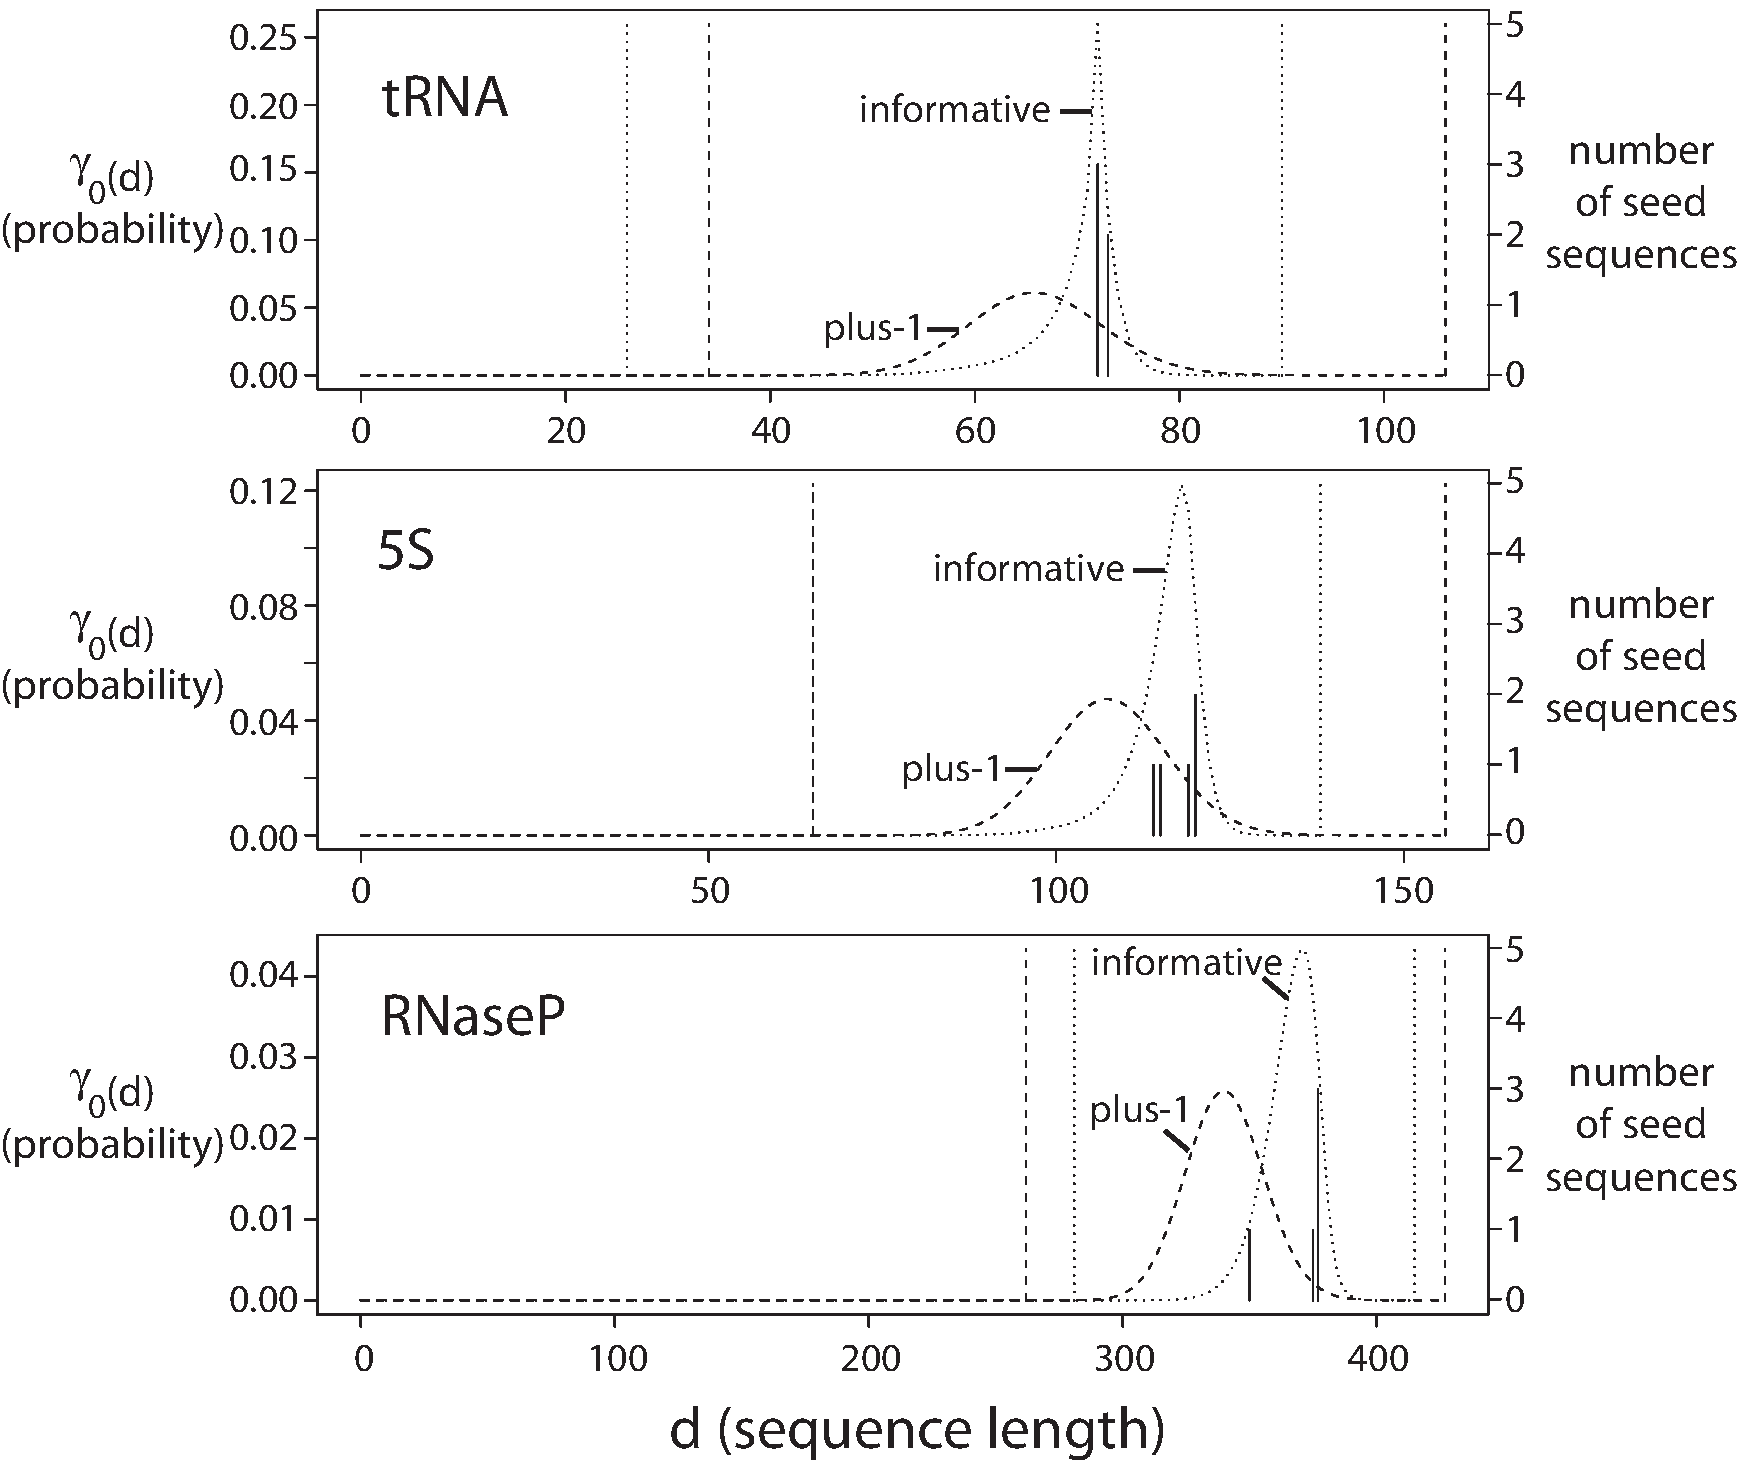
\includegraphics[width=6in,angle=0]{figs/3fam_bands}
    \caption{\textbf{Effect of transition priors on band calculation.}
      Predicted and actual target lengths are shown for three CMs
      built from alignments of five tRNA, 5S rRNA, and RNaseP
      sequences, which are about 75, 120, and 380 residues long,
      respectively.  Solid vertical lines represent the actual lengths
      of the sequences in each alignment, corresponding with the right
      vertical axis labels. Dashed and dotted curves show QDB
      calculations for $\gamma_0(d)$ for the root state of each model,
      for uninformative versus informative Dirichlet priors,
      respectively.  Dashed and dotted vertical lines show the band
      bounds ($d_{\mbox{min}}(0)$ (left) and $d_{\mbox{max}}(0)$
      (right)) derived from the $\gamma_0(d)$ distributions using
      $\beta = 10^{-7}$. The uninformative plus-one prior results in
      consistent underprediction of target sequence lengths, with a
      broad distribution. The new informative priors produce tighter
      distributions that are centered on the actual subsequence
      lengths. We observe the same result for all other states
      (data not shown).}
    \label{fig:bands}
  \end{center}
\end{figure}

% This is \ref{fig:bands}
\fi

The training data for transition priors consisted of the 381 seed
alignments in the Rfam database, version 6.1
\cite{Griffiths-Jones05}. For each alignment, we built CM structures
by \textsc{infernal}'s default procedure, and collected weighted
counts of observed transitions in the implied parse trees of the
training sequences. Considering all possible combinations of pairs of
adjacent node types, there are 73 possible distinct types of
transition probability distributions in CMs. To reduce this parameter
space, we tied these 73 distributions into 36 groups by assuming that
certain distributions were effectively equivalent.  36 Dirichlet
densities were then estimated from these pooled counts by maximum
likelihood as described in \cite{Sjolander96}, with the exception that
we optimize by conjugate gradient descent \cite{Press93} rather than
by expectation-maximization (EM).  The results, including the
Dirichlet parameters, are given in Table~\ref{tbl:transitions}.  Using
these priors for transition probability parameter estimation results
in an improvement in the utility of QDB calculations, often yielding
tighter, yet accurate subsequence length distributions, as illustrated
by anecdotal example in Figure~\ref{fig:bands}.

\ifdraft
\renewcommand{\baselinestretch}{1.0}
\begin{table}
\renewcommand{\tabcolsep}{0.7em}
\tiny
\begin{center}
%\begin{tabular}{|r|r|l|l|l||l|r||l|r||l|r||l|r||l|r||l|r||} \hline
\begin{tabular}{|rr|rr|cc|c|c|cc|cc|cc|cc|cc|cc|} \cline{1-6} \cline{8-20}
%\multicolumn{5}{c}{} & \multicolumn{2}{|c|}{1} & \multicolumn{2}{|c|}{2} & \multicolumn{2}{|c|}{3} & \multicolumn{2}{|c|}{4} & \multicolumn{2}{|c|}{5} & \multicolumn{2}{|c|}{6} \\ \cline{1-17}
\multicolumn{1}{|c}{dist} & \multicolumn{1}{c|}{tied} &
  \multicolumn{1}{c}{dist} & \multicolumn{1}{c|}{grp} & node & next &
  & \multicolumn{13}{|c|}{Dirichlet $\alpha$ parameters} \\ %\cline{8-20}
%\multicolumn{1}{|c}{\#} & \multicolumn{1}{c|}{\#} & \multicolumn{1}{c}{counts} & \multicolumn{1}{c|}{counts} & state & node & & $|\alpha|$ & $a_1$ &
%  $\frac{\alpha_{a_1}}{|\alpha|}$ & $a_2$ & $\frac{\alpha_{a_2}}{|\alpha|}$ & $a_3$ &
%  $\frac{\alpha_{a_3}}{|\alpha|}$ & $a_4$ & $\frac{\alpha_{a_4}}{|\alpha|}$ & $a_5$ &
%  $\frac{\alpha_{a_5}}{|\alpha|}$ & $a_6$ & $\frac{\alpha_{a_6}}{|\alpha|}$ \\
%  \cline{1-6} \cline {8-20} 
\multicolumn{1}{|c}{\#} & \multicolumn{1}{c|}{to} & \multicolumn{1}{c}{counts} & \multicolumn{1}{c|}{counts} & state & node & & $|\alpha|$ & $a$ &
  $\frac{\alpha_{a}}{|\alpha|}$ & $a$ & $\frac{\alpha_{a}}{|\alpha|}$ & $a$ &
  $\frac{\alpha_{a}}{|\alpha|}$ & $a$ & $\frac{\alpha_{a}}{|\alpha|}$ & $a$ &
  $\frac{\alpha_{a}}{|\alpha|}$ & $a$ & $\frac{\alpha_{a}}{|\alpha|}$ \\
  \cline{1-6} \cline {8-20} 

1   &    & 6     & 11    & MATP\_MP & BIF  & & 0.5509  & IL & 0.1229 & IR & 0.0001 & B  & 0.8770 &    &        &    &  &  &  \\  
2   &    & 7023  & 7119  & MATP\_MP & MATP & & 7.2986  & IL & 0.0023 & IR & 0.0024 & MP & 0.9816 & ML & 0.0056 & MR & 0.0046 & D & 0.0035 \\  
3   &    & 1600  & 1830  & MATP\_MP & MATL & & 1.5914  & IL & 0.0179 & IR & 0.0155 & ML & 0.9200 & D  & 0.0466 &    &  &  &  \\  
4   &    & 145   & 195   & MATP\_MP & MATR & & 1.9038  & IL & 0.0173 & IR & 0.0073 & MR & 0.8903 & D  & 0.0852 &    &  &  &  \\  
5   & 1  & 2     & 11    & MATP\_MP & END  & & 0.5509  & IL & 0.1229 & IR & 0.0001 & E  & 0.8770 &    &        &    &  &  &  \\  
6*  &    & 1     & 2     & MATP\_ML & BIF  & & 3.0000  & IL & 0.3333 & IR & 0.3333 & B  & 0.3333 &    &        &    &  &  &  \\  
7   &    & 577   & 577   & MATP\_ML & MATP & & 0.6941  & IL & 0.0131 & IR & 0.0103 & MP & 0.4032 & ML & 0.4983 & MR & 0.0115 & D & 0.0636 \\  
8   &    & 133   & 133   & MATP\_ML & MATL & & 0.9316  & IL & 0.0739 & IR & 0.0651 & ML & 0.7038 & D  & 0.1571 &    &  &  &  \\  
9   &    & 15    & 15    & MATP\_ML & MATR & & 0.3272  & IL & 0.1884 & IR & 0.0432 & MR & 0.4082 & D  & 0.3602 &    &  &  &  \\  
10* & 6  & 1     & 2     & MATP\_ML & END  & & 3.0000  & IL & 0.3333 & IR & 0.3333 & E  & 0.3333 &    &        &    &  &  &  \\  
11* &    & 1     & 2     & MATP\_MR & BIF  & & 3.0000  & IL & 0.3333 & IR & 0.3333 & B  & 0.3333 &    &        &    &  &  &  \\  
12  &    & 531   & 531   & MATP\_MR & MATP & & 0.7987  & IL & 0.0079 & IR & 0.0190 & MP & 0.3241 & ML & 0.0193 & MR & 0.5631 & D & 0.0666 \\  
13  &    & 151   & 151   & MATP\_MR & MATL & & 0.6933  & IL & 0.0357 & IR & 0.0699 & ML & 0.3066 & D  & 0.5879 &    &  &  &  \\  
14  &    & 15    & 15    & MATP\_MR & MATR & & 0.3574  & IL & 0.0582 & IR & 0.0002 & MR & 0.7629 & D  & 0.1787 &    &  &  &  \\  
15* & 11 & 1     & 2     & MATP\_MR & END  & & 3.0000  & IL & 0.3333 & IR & 0.3333 & E  & 0.3333 &    &        &    &  &  &  \\  
16* &    & 0     & 2     & MATP\_D  & BIF  & & 3.0000  & IL & 0.3333 & IR & 0.3333 & B  & 0.3333 &    &        &    &  &  &  \\  
17  &    & 575   & 575   & MATP\_D  & MATP & & 0.5450  & IL & 0.0019 & IR & 0.0047 & MP & 0.0857 & ML & 0.0534 & MR & 0.0528 & D & 0.8015 \\  
18  &    & 149   & 149   & MATP\_D  & MATL & & 0.5831  & IL & 0.0421 & IR & 0.0526 & ML & 0.2080 & D  & 0.6973 &    &  &  &  \\  
19  &    & 14    & 14    & MATP\_D  & MATR & & 0.1164  & IL & 0.0001 & IR & 0.0001 & MR & 0.2439 & D  & 0.7559 &    &  &  &  \\  
20* & 16 & 2     & 2     & MATP\_D  & END  & & 3.0000  & IL & 0.3333 & IR & 0.3333 & E  & 0.3333 &    &        &    &  &  &  \\  
21  &    & 2     & 4     & MATP\_IL & BIF  & & 1.4397  & IL & 0.6553 & IR & 0.0445 & B  & 0.3002 &    &        &    &  &  &  \\  
22  &    & 121   & 126   & MATP\_IL & MATP & & 0.9402  & IL & 0.1673 & IR & 0.1394 & MP & 0.5904 & ML & 0.0443 & MR & 0.0259 & D & 0.0327 \\  
23  &    & 114   & 119   & MATP\_IL & MATL & & 0.8046  & IL & 0.3108 & IR & 0.1936 & ML & 0.4610 & D  & 0.0346 &    &  &  &  \\  
24  &    & 14    & 15    & MATP\_IL & MATR & & 1.0926  & IL & 0.1419 & IR & 0.0501 & MR & 0.6538 & D  & 0.1541 &    &  &  &  \\  
25  & 21 & 2     & 4     & MATP\_IL & END  & & 1.4397  & IL & 0.6553 & IR & 0.0445 & E  & 0.3002 &    &        &    &  &  &  \\  
26  &    & 1     & 31    & MATP\_IR & BIF  & & 0.9361  & IR & 0.2827 & B  & 0.7173 &    &        &    &        &    &  &  &  \\  
27  &    & 145   & 227   & MATP\_IR & MATP & & 1.5494  & IR & 0.1884 & MP & 0.7090 & ML & 0.0165 & MR & 0.0588 & D  & 0.0273 &  &  \\  
28  &    & 129   & 701   & MATP\_IR & MATL & & 1.6332  & IR & 0.3681 & ML & 0.5752 & D  & 0.0566 &    &        &    &  &  &  \\  
29  &    & 8     & 160   & MATP\_IR & MATR & & 1.2428  & IR & 0.2633 & MR & 0.6809 & D  & 0.0558 &    &        &    &  &  &  \\  
30  & 26 & 0     & 31    & MATP\_IR & END  & & 0.9361  & IR & 0.2827 & E  & 0.7173 &    &        &    &        &    &  &  &  \\  
31  &    & 108   & 1130  & MATL\_ML & BIF  & & 1.2298  & IL & 0.0078 & B  & 0.9922 &    &        &    &        &    &  &  &  \\  
32  &    & 420   & 1319  & MATL\_ML & MATP & & 2.4162  & IL & 0.0132 & MP & 0.9520 & ML & 0.0150 & MR & 0.0129 & D  & 0.0070 &  &  \\  
33  &    & 19013 & 19371 & MATL\_ML & MATL & & 1.8632  & IL & 0.0082 & ML & 0.9711 & D  & 0.0207 &    &        &    &  &  &  \\  
34  &    & 859   & 6692  & MATL\_ML & MATR & & 72.1283 & IL & 0.0058 & MR & 0.9755 & D  & 0.0187 &    &        &    &  &  &  \\  
35  & 31 & 801   & 1130  & MATL\_ML & END  & & 1.2298  & IL & 0.0078 & E  & 0.9922 &    &        &    &        &    &  &  &  \\  
36  &    & 28    & 172   & MATL\_D  & BIF  & & 6.8008  & IL & 0.0029 & B  & 0.9971 &    &        &    &        &    &  &  &  \\  
37  &    & 103   & 103   & MATL\_D  & MATP & & 0.7288  & IL & 0.0321 & MP & 0.5730 & ML & 0.0536 & MR & 0.1654 & D  & 0.1758 &  &  \\  
38  &    & 3152  & 3152  & MATL\_D  & MATL & & 0.4101  & IL & 0.0138 & ML & 0.3105 & D  & 0.6756 &    &        &    &  &  &  \\  
39  &    & 154   & 154   & MATL\_D  & MATR & & 0.6736  & IL & 0.0203 & MR & 0.6014 & D  & 0.3782 &    &        &    &  &  &  \\  
40  & 36 & 144   & 172   & MATL\_D  & END  & & 6.8008  & IL & 0.0029 & E  & 0.9971 &    &        &    &        &    &  &  &  \\  
41  & 26 & 13    & 31    & MATL\_IL & BIF  & & 0.9361  & IL & 0.2827 & B  & 0.7173 &    &        &    &        &    &  &  &  \\  
42  & 27 & 35    & 227   & MATL\_IL & MATP & & 1.5494  & IL & 0.1884 & MP & 0.7090 & ML & 0.0588 & MR & 0.0165 & D  & 0.0273 &  &  \\  
43  & 28 & 549   & 701   & MATL\_IL & MATL & & 1.6332  & IL & 0.3681 & ML & 0.5752 & D  & 0.0566 &    &        &    &  &  &  \\  
44  & 29 & 45    & 160   & MATL\_IL & MATR & & 1.2428  & IL & 0.2633 & MR & 0.6809 & D  & 0.0558 &    &        &    &  &  &  \\  
45  & 26 & 0     & 31    & MATL\_IL & END  & & 0.9361  & IL & 0.2827 & E  & 0.7173 &    &        &    &        &    &  &  &  \\  
46  & 31 & 206   & 1130  & MATR\_MR & BIF  & & 1.2298  & IR & 0.0078 & B  & 0.9922 &    &        &    &        &    &  &  &  \\  
47  & 32 & 848   & 1319  & MATR\_MR & MATP & & 2.4162  & IR & 0.0132 & MP & 0.9520 & ML & 0.0150 & MR & 0.0129 & D  & 0.0070 &  &  \\  
48  & 34 & 5833  & 6692  & MATR\_MR & MATR & & 2.1283  & IR & 0.0058 & MR & 0.9755 & D  & 0.0187 &    &        &    &  &  &  \\  
49  &    & 39    & 39    & MATR\_D  & BIF  & & 0.4664  & IR & 0.0463 & B  & 0.9537 &    &        &    &        &    &  &  &  \\  
50  &    & 176   & 176   & MATR\_D  & MATP & & 0.8689  & IR & 0.0245 & MP & 0.6126 & ML & 0.1269 & MR & 0.0471 & D  & 0.1890 &  &  \\  
51  &    & 771   & 771   & MATR\_D  & MATR & & 0.4869  & IR & 0.0119 & MR & 0.3373 & D  & 0.6507 &    &        &    &  &  &  \\  
52  & 26 & 15    & 31    & MATR\_IR & BIF  & & 0.9361  & IR & 0.2827 & B  & 0.7173 &    &        &    &        &    &   &  &  \\  
53  & 27 & 39    & 227   & MATR\_IR & MATP & & 1.5494  & IR & 0.1884 & MP & 0.7090 & ML & 0.0165 & MR & 0.0588 & D  & 0.0273 &  &  \\  
54  & 29 & 107   & 160   & MATR\_IR & MATR & & 1.2428  & IR & 0.2633 & MR & 0.6809 & D  & 0.0558 &    &        &    &  &  &  \\  
%55 &    &       &       & BEGL\_S  & BIF  & & 1.0000  & B  & 1.0000 &    &        &    &        &    &        &    &  &  &  \\  
55  &    & 338   & 338   & BEGL\_S  & MATP & & 5.0422  & MP & 0.9579 & ML & 0.0121 & MR & 0.0183 & D  & 0.0117 &    &   &  &  \\  
56  & 31 & 15    & 1130  & BEGR\_S  & BIF  & & 1.2298  & IL & 0.0078 & B  & 0.9922 &    &        &    &        &    &  &  &  \\  
57  & 32 & 51    & 1319  & BEGR\_S  & MATP & & 2.4162  & IL & 0.0132 & MP & 0.9520 & ML & 0.0150 & MR & 0.0129 & D  & 0.0070 &  &  \\  
58  & 33 & 358   & 19371 & BEGR\_S  & MATL & & 1.8632  & IL & 0.0082 & ML & 0.9711 & D  & 0.0207 &    &        &    &  &  &  \\  
59  & 26 & 2     & 31    & BEGR\_IL & BIF  & & 0.9361  & IL & 0.2827 & B  & 0.7173 &    &        &    &        &    &   &  &  \\  
60  & 27 & 3     & 227   & BEGR\_IL & MATP & & 1.5494  & IL & 0.1884 & MP & 0.7090 & ML & 0.0588 & MR & 0.0165 & D  & 0.0273 &  &  \\  
61  & 28 & 19    & 701   & BEGR\_IL & MATL & & 1.6332  & IL & 0.3681 & ML & 0.5752 & D  & 0.0566 &    &        &    &  &  &  \\  
62  & 1  & 3     & 11    & ROOT\_S  & BIF  & & 0.5509  & IL & 0.1229 & IR & 0.0001 & B  & 0.8770 &    &        &    &  &  &  \\  
63  & 2  & 96    & 7119  & ROOT\_S  & MATP & & 7.2986  & IL & 0.0023 & IR & 0.0024 & MP & 0.9816 & ML & 0.0056 & MR & 0.0046 & D & 0.0035 \\  
64  & 3  & 230   & 1830  & ROOT\_S  & MATL & & 1.5914  & IL & 0.0179 & IR & 0.0155 & ML & 0.9200 & D  & 0.0466 &    &  &  &  \\  
65  & 4  & 50    & 195   & ROOT\_S  & MATR & & 1.9038  & IL & 0.0173 & IR & 0.0073 & MR & 0.8903 & D  & 0.0852 &    &  &  &  \\  
66  & 21 & 0     & 4     & ROOT\_IL & BIF  & & 1.4397  & IL & 0.6553 & IR & 0.0445 & B  & 0.3002 &    &        &    &  &  &  \\  
67  & 22 & 5     & 126   & ROOT\_IL & MATP & & 0.9402  & IL & 0.1673 & IR & 0.1394 & MP & 0.5904 & ML & 0.0443 & MR & 0.0259 & D & 0.0327 \\  
68  & 23 & 5     & 119   & ROOT\_IL & MATL & & 0.8046  & IL & 0.3108 & IR & 0.1936 & ML & 0.4610 & D  & 0.0346 &    &  &  &  \\  
69  & 24 & 1     & 15    & ROOT\_IL & MATR & & 1.0926  & IL & 0.1419 & IR & 0.0501 & MR & 0.6538 & D  & 0.1541 &    &  &  &  \\  
70  & 26 & 0     & 31    & ROOT\_IR & BIF  & & 0.9361  & IR & 0.2827 & B  & 0.7173 &    &        &    &        &    &  &  &  \\  
71  & 27 & 5     & 227   & ROOT\_IR & MATP & & 1.5494  & IR & 0.1884 & MP & 0.7090 & ML & 0.0165 & MR & 0.0588 & D  & 0.0273 &  &  \\  
72  & 28 & 4     & 701   & ROOT\_IR & MATL & & 1.6332  & IR & 0.3681 & ML & 0.5752 & D  & 0.0566 &    &        &    &  &  &  \\  
73  & 29 & 0     & 160   & ROOT\_IR & MATR & & 1.2428  & IR & 0.2633 & MR & 0.6809 & D  & 0.0558 &    &        &    &  &  &  \\   \cline{1-6} \cline {8-20} 
\end{tabular}
\end{center}

\normalfont\rmfamily
\caption{\textbf{Dirichlet priors for transitions.}  ``dist \#''=
  index for the 73 different types of transition distributions in CMs;
  asterisks mark six distributions which had very few observed counts
  even after tying into groups, and for which we assigned a uniform
  plus-one Laplace prior. ``tied to''= if an index is shown in this
  column, this distribution was estimated in a group (pooling observed
  counts) with the indicated distribution.  ``dist counts''= total
  counts observed for this distribution in the training data, before
  pooling into groups. ``grp counts''= total counts for a group of one
  or more pooled distributions; this is the size of the training data
  sets for 36 different single-component Dirichlet priors.  ``node
  state''= unique CM state type the transition is from. 
  ``next node''= the node type that the transitions are going to.
  The codes for node types and state types in a CM are more fully
  explained in \cite{Eddy02b}.
}
\label{tbl:transitions}
\end{table}
\renewcommand{\baselinestretch}{1.5}

% This is {tbl:transitions}
\fi

We also estimated informative mixture Dirichlet density priors for
emission probabilities.  Emission probabilities have no effect on QDB,
but informative emission priors should improve sensitivity and
specificity of CM searches, as they do for profile hidden Markov
models \cite{BrownM93,Sjolander96}. We collected filtered counts of
aligned single-stranded residues and base-pairs from annotated
ribosomal RNA alignments from four alignments in the 2002 version of
the European Ribosomal RNA Database \cite{Wuyts01, Wuyts02}: large
subunit rRNA (LSU), bacterial/archaeal/plastid small subunit rRNA
(SSU-bap), eukaryotic SSU rRNA (SSU-euk), and mitochondrial SSU rRNA
(SSU-mito). These alignments were filtered, removing sequences in
which either less than 40\% of the base paired positions are present
or more than 5\% of the nucleotides are ambiguous, and removing
selected sequences based on single-linkage-clustering such that no two
sequences in a filtered alignment were greater than 80\% identical (in
order to remove closely related sequences). Summary statistics for the
filtered alignments and collected counts in the training dataset are
given in Table~\ref{tbl:emissioncounts}. These data were used to
estimate a nine-component Dirichlet mixture prior for base pairs, and
an eight-component Dirichlet mixture prior for single stranded
residues. The base pair prior is given in
Table~\ref{tbl:basepairs}, and the singlet residue prior is given in
Table~\ref{tbl:singlets}. 

The reason to use two different datasets to estimate transition versus
emission priors is the following. Rfam provides many different
structural RNA alignments, but of uneven quality and varying depth
(number of sequences). The European rRNA database provides a small
number of different RNA alignments, but of high quality and great
depth.  A transition prior training set should be maximally diverse,
so as not to bias any transition types toward any particular RNA
structure, so we used the 381 different Rfam alignments for
transitions.  Emission prior estimation, in contrast, improves with
alignment depth and accuracy, but does not require broad structural
diversity per se, so we used rRNA data for emissions.

Inspection of the Dirichlet $\alpha$ parameters shows sensible
trends. In the transition priors, transitions between main (consensus)
states are now favored (higher $\alpha$ values) relative to insertions
and deletions.  In the base pair emission mixture prior, all
components favor Watson-Crick and G-U pairs, with different components
preferring different proportions of pairs in a particular covarying
aligned column (for instance, component 1 likes all four Watson-Crick
pairs, component 2 describes covarying conservation of CG,UA,UG pairs,
and component 3 specifically likes conserved CG pairs), and the mean
$\alpha$ parameters prefer GC/CG pairs over AU/UA pairs. In the
singlet emission mixture prior, some components are capturing strongly
conserved residues (component 1 favors conserved U's, for example)
while other components favor more variation (components 4 and 5, for
example), and the marginal $\alpha$ parameters show a strong A bias,
reflecting the known bias for adenine in single-stranded positions of
structural RNAs (especially ribosomal RNAs).

There is redundancy between some components (notably 5 and 8
in the base pair mixture and 2, 3 and 8 in the singlet mixture). This
is typical for statistical mixture estimation, which (unlike, say,
principal components analysis) does not guarantee independence between
components. The decision to use nine pair and eight singlet components
was empirical, as these priors performed better than priors with fewer
components on the benchmark we describe below (data not shown).

Note that all singlet positions are modeled with one singlet mixture
prior distribution, and all base pairs are modeled with one base pair
mixture prior. These priors do not distinguish between singlet
residues in different types of loops, for example, nor between a
stem-closing base pair versus other base pairs. In the future it may
prove advantageous to adopt more complex priors to capture 
effects of structural context on base pair and singlet residue
preference.

\ifdraft
%%%%%%%%%%%%%%%%%%%%%%%%%%%%%%%%%%%%%%%%%%%%%%%%%%%%%%%%%%%%%%%%%%%%%%%
% The emission prior alignment counts
% this table is in my rotation lab presentation ./emit_priors_revisited/nawrocki_dirichlet.pdf
%\renewcommand{\baselinestretch}{1.0}
\begin{table}
%\normalfont\ttfamily
\begin{center}
\begin{tabular}{lrrrrrrr} 
& & \# filtered & \# aln & \# consensus & \# consensus & base pair & SS \\
alignment & \# seqs & seqs & columns & base pairs  & SS columns & counts & counts \\ \hline
LSU      & 1551  & 139  & 7270 & 601 & 1532  & 65229 & 180558  \\
SSU bap  & 12773 & 254  & 2653 & 421 & 680   & 97834 & 153565  \\
SSU euk  & 7151  & 207  & 4558 & 407 & 959   & 72521 & 174260  \\
SSU mito & 1039  & 107  & 3791 & 216 & 524   & 19803 & 56510   \\ 
%\multicolumn{8}{l}{bap: contains bacterial, archaeal and plastid
%  sequences} \\
\end{tabular}
\end{center}
\caption{\textbf{Summary statistics for the dataset used for emission prior
    estimation.} ``SS'' = single-stranded.} 
\label{tbl:emissioncounts}
\end{table}

% This is tbl:emissioncounts
\fi

\ifdraft
%%%%%%%%%%%%%%%%%%%%%%%%%%%%%%%%%%%%%%%%%%%%%%%%%%%%%%%%%%%%%%%%%%%%%%%
% 04.10.06 The priors tables.
% these were sequestered to the supplementary material in draft 2,
% but they're back to the main document for draft 3.
%
% These tables were generated by dchlet2latex_d3.pl revision 369, in 
% in ~nawrocki/notebook/6_0404_inf_banded_mscript_d3/latex/dchlet_tbls_dir/:
%
% $ perl dchlet2latex_d3.pl dchlet56.prior 041006
% generates 041006_bp_priors.tex, 041006_sing_priors.tex and
%           041006_trans_priors.tex, which include the following
%           three tables (in slightly different format, I tweaked
%           them to get these).
%%%%%%%%%%%%%%%%%%%%%%%%%%%%%%%%%%%%%%%%%%%%%%%%%%%%%%%%%%%%%%%%%%%%%%%
% Base pair emission priors. 041006_bp_priors.tex (with modifications)

\begin{table}
%\normalfont\ttfamily
\footnotesize
\begin{center}
\begin{tabular}{|c|c|c|c|c|c|c|c|c|c|c|} \hline
\multicolumn{2}{|c|}{component $i$} & 1 & 2 & 3 & 4 & 5 & 6 & 7 & 8 & 9 \\
\multicolumn{2}{|c|}{$q_i$} & 0.0305 & 0.0703 & 0.1185 & 0.1810 & 0.1888 & 0.1576 & 0.0417 & 0.0959 & 0.1156 \\
\multicolumn{2}{|c|}{$|\alpha|$} & 14.3744 & 2.9920 & 26.2757 & 0.5342 &
4.2716 & 13.3232 & 33.8619 & 22.2258 & 33.1991 \\ \hline 
\multicolumn{11}{c}{} \\ \hline

$ab$ & mean $\alpha$ & $\frac{\alpha_{ab}}{|\alpha|}$ & $\frac{\alpha_{ab}}{|\alpha|}$ & $\frac{\alpha_{ab}}{|\alpha|}$ & $\frac{\alpha_{ab}}{|\alpha|}$ & $\frac{\alpha_{ab}}{|\alpha|}$ & $\frac{\alpha_{ab}}{|\alpha|}$ & $\frac{\alpha_{ab}}{|\alpha|}$ & $\frac{\alpha_{ab}}{|\alpha|}$ & $\frac{\alpha_{ab}}{|\alpha|}$ \\ \hline 
AA & 0.0063 & 0.0398 & 0.0390 & 0.0011 & 0.0017 & 0.0005 & 0.0062 & 0.0064 & 0.0058 & 0.0002 \\  
AC & 0.0092 & 0.0421 & 0.0176 & 0.0009 & 0.0152 & 0.0018 & 0.0125 & 0.0115 & 0.0051 & 0.0046 \\  
AG & 0.0052 & 0.0381 & 0.0226 & 0.0046 & 0.0034 & 0.0008 & 0.0032 & 0.0040 & 0.0053 & 0.0001 \\  
AU & \textbf{0.1663} & \textbf{0.1092} & 0.0864 & 0.0194 & \textbf{0.2138} & \textbf{0.1464} & \textbf{0.2563} & \textbf{0.7360} & \textbf{0.1295} & 0.0404 \\  
& & & & & & & & & & \\
CA & 0.0086 & 0.0412 & 0.0510 & 0.0054 & 0.0027 & 0.0044 & 0.0018 & 0.0030 & 0.0138 & 0.0002 \\  
CC & 0.0038 & 0.0327 & 0.0115 & 0.0030 & 0.0001 & 0.0003 & 0.0036 & 0.0039 & 0.0035 & 0.0041 \\  
CG & \textbf{0.2412} & \textbf{0.1007} & \textbf{0.1392} & \textbf{0.8310} & \textbf{0.1359} & \textbf{0.3211} & 0.0889 & 0.0340 & \textbf{0.2870} & 0.0147 \\  
CU & 0.0066 & 0.0418 & 0.0172 & 0.0027 & 0.0104 & 0.0019 & 0.0045 & 0.0076 & 0.0052 & 0.0003 \\  
& & & & & & & & & & \\
GA & 0.0061 & 0.0362 & 0.0266 & 0.0002 & 0.0074 & 0.0002 & 0.0058 & 0.0045 & 0.0042 & 0.0021 \\  
GC & \textbf{0.2547} & \textbf{0.1299} & 0.0544 & 0.0206 & \textbf{0.1786} & \textbf{0.1613} & \textbf{0.4079} & 0.0945 & \textbf{0.1155} & \textbf{0.8858} \\  
GG & 0.0063 & 0.0327 & 0.0142 & 0.0045 & 0.0091 & 0.0005 & 0.0072 & 0.0023 & 0.0044 & 0.0030 \\  
GU & 0.0567 & 0.0811 & 0.0412 & 0.0049 & \textbf{0.1355} & 0.0451 & 0.0668 & 0.0303 & 0.0356 & 0.0218 \\  
& & & & & & & & & & \\
UA & \textbf{0.1571} & \textbf{0.1063} & \textbf{0.3085} & 0.0672 & \textbf{0.1856} & \textbf{0.2293} & 0.0902 & 0.0363 & \textbf{0.3108} & 0.0151 \\  
UC & 0.0063 & 0.0477 & 0.0263 & 0.0006 & 0.0048 & 0.0002 & 0.0056 & 0.0042 & 0.0060 & 0.0038 \\  
UG & 0.0543 & 0.0746 & \textbf{0.1054} & 0.0317 & 0.0807 & 0.0814 & 0.0299 & 0.0120 & 0.0551 & 0.0032 \\  
UU & 0.0114 & 0.0459 & 0.0389 & 0.0022 & 0.0151 & 0.0048 & 0.0098 & 0.0095 & 0.0133 & 0.0008 \\ \hline 
\end{tabular}
\end{center}

\normalfont\rmfamily
\caption{\textbf{Parameters of the 9 component Dirichlet mixture
    emission prior for base pairs.} $q_i =$ mixture coefficient for
    component $i$. Normalized $\alpha$ values $> 0.10$ are in bold
    face.}
\label{tbl:basepairs}
\end{table}

% This is tbl:basepairs
\fi

\ifdraft
%%%%%%%%%%%%%%%%%%%%%%%%%%%%%%%%%%%%%%%%%%%%%%%%%%%%%%%%%%%%%%%%%%%%%%%
% Singlet emission priors. 041006_sing_priors.tex (with modifications)
\begin{table}
%\normalfont\ttfamily
\footnotesize
\begin{center}
\begin{tabular}{|c|c|c|c|c|c|c|c|c|c|c|} \hline
\multicolumn{2}{|c|}{component $i$} & 1 & 2 & 3 & 4 & 5 & 6 & 7 & 8 \\
\multicolumn{2}{|c|}{$q_i$} & 0.0851 & 0.0159 & 0.1020 & 0.4160 & 0.0745 & 0.0554 & 0.1184 & 0.1327 \\  
\multicolumn{2}{|c|}{$|\alpha|$} & 15.4467 & 154.4640 & 180.2862 & 5.4562 & 0.2199 & 16.4089 & 13.4592 & 19.9059 \\ \hline 
\multicolumn{10}{c}{} \\ \hline

$a$ & mean $\alpha$ & $\frac{\alpha_a}{|\alpha|}$ & $\frac{\alpha_a}{|\alpha|}$ & $\frac{\alpha_a}{|\alpha|}$ & $\frac{\alpha_a}{|\alpha|}$ & $\frac{\alpha_a}{|\alpha|}$ & $\frac{\alpha_a}{|\alpha|}$ & $\frac{\alpha_a}{|\alpha|}$ & $\frac{\alpha_a}{|\alpha|}$ \\ \hline 
A & \textbf{0.3951} & 0.0373 & \textbf{0.9961} & \textbf{0.9787} & \textbf{0.3109} & \textbf{0.3383} & 0.0375 & 0.0864 & \textbf{0.8247} \\  
C & \textbf{0.1635} & 0.0490 & 0.0015 & 0.0052 & \textbf{0.2067} & \textbf{0.1782} & \textbf{0.8916} & 0.0303 & 0.0493 \\  
G & \textbf{0.2041} & 0.0220 & 0.0023 & 0.0072 & \textbf{0.1751} & \textbf{0.2905} & 0.0182 & \textbf{0.8313} & 0.0569 \\  
U & \textbf{0.2372} & \textbf{0.8917} & 0.0000 & 0.0090 & \textbf{0.3073} & \textbf{0.1930} & 0.0527 & 0.0519 & 0.0691 \\ \hline 


\end{tabular}
\end{center}

\normalfont\rmfamily
\caption{\textbf{Parameters of the 8 component Dirichlet mixture
    emission prior for singlets.} $q_i =$ mixture coefficient for
    component $i$. Normalized $\alpha$ values $> 0.10$ are in bold
    faced type ($0.10$ was arbitrarily chosen to highlight higher values).}
\label{tbl:singlets}
\end{table}

% This is tbl:singlets
\fi

In another step to increase sensitivity and specificity of the
program, we adopted the ``entropy weighting'' technique described for
profile HMMs \cite{Karplus98} for estimating the total effective
sequence number for an input query alignment. This is an \emph{ad hoc}
method for reducing the information content per position of a model,
which helps a model that has been trained on closely related sequences
to recognize distantly related homologues \cite{Altschul91}. In
entropy weighting, one reduces the total effective sequence number
(which would normally be the actual number of sequences in the input
alignment), thereby increasing the influence of the Dirichlet priors,
flattening the transition and emission distributions, and reducing the
overall information content. We approximate a model's entropy as the
mean entropy per consensus residue, as follows. Let $C$ be the set of
all MATP\_MP states emitting consensus base pairs ($a$,$b$), and let
$D$ be the set of all MATL\_ML and MATR\_MR states emitting consensus
singlets ($a$); the entropy is then calculated as:

\[
\frac{ \sum_{v \in C} - \sum_{a,b} e_v(a,b) \log e_v(a,b) -
       \sum_{v \in D} \sum_{a}   e_v(a)   \log e_v(a)}
{2|C| + |D|}
\]

For each input multiple alignment, the effective sequence number is
set (by bracketing and binary search) so as to obtain a specified
target entropy.  The target entropy for \textsc{infernal} is a free
parameter, which we optimized on the benchmark described below to
identify our default value of 1.46 bits.

\subsection{Benchmarking}

To assess the effect of QDB, informative priors, and entropy weighting
on the speed, sensitivity, and specificity of RNA similarity searches,
we designed a benchmark based on the Rfam database
\cite{Griffiths-Jones05}. The benchmark was designed so that we would
test many RNA query/target pairs, with each query consisting of a
given RNA sequence alignment, and each target consisting of a
distantly related RNA homolog buried in a context of a random
genome-like background sequence.

We started with seed alignments from Rfam version 7.0. In each
alignment, sequences shorter than 70\% the median length were removed.
We clustered the sequences in each family by single-linkage-clustering
by \% identity (as calculated from the given Rfam alignment), then
split the clusters such that the training set and test sequences
satisfied three conditions: 1) no training/test sequence pair is more
than 60\% identical; 2) no test sequence pair is greater than 70\%
identical; 3) at least 5 sequences are in the training set.  Fifty-one
families satisfy these criteria (listed in Table~\ref{tbl:rmark}),
giving us 51 different query alignments (containing 5 to 1080
sequences each) and 450 total test sequences (from 1 to 66 per query).
We embedded the test sequences in a one megabase ``pseudo-genome''
consisting of twenty 50 kilobase ``chromosomes'', generated as
independent, identically distributed (iid) random sequences with
uniform base frequencies.  The 450 test sequences were embedded into
this sequence by replacement, by randomly choosing a chromosome,
orientation, and start position, and disallowing overlaps between test
sequences. The total length of the 450 test sequences is 101,855 nt,
leaving 898,145 nt of random background sequence.

\ifdraft
%  Merge table 6+7 here: ranked by length as in tbl 7
%
% <Rfam ID>   - from tbl7
% <family>
%
% <# query>   - from tbl6
% <# test>
%
% avg query len  - from tbl7 (rearranged a bit)
% W
% standard time
% QDB time (1e-7)
% speedup
%
% MER             -from tbl6 (delete TP, it's redundant)
% FP
% FN
% threshold (bits)

\renewcommand{\baselinestretch}{1.0}
\begin{table}
\scriptsize
\begin{center}
\begin{tabular}{|ll|rr|rr|r|rr|rrrr|} \hline
\multicolumn{1}{|c}{Rfam 7.0} & \multicolumn{1}{c|}{family} &
\multicolumn{1}{c}{\#} & \multicolumn{1}{c|}{\#} &
\multicolumn{1}{c}{avg len} & \multicolumn{1}{c|}{} &
\multicolumn{1}{c}{non-banded} & \multicolumn{2}{|c|}{QDB
    ($\beta=10^{-7}$)} &  \multicolumn{3}{|c}{} & \multicolumn{1}{c|}{thr} \\ 
\multicolumn{1}{|c}{ID} & \multicolumn{1}{c|}{name} &
\multicolumn{1}{c}{query} & \multicolumn{1}{c|}{test} &
\multicolumn{1}{c}{query} & \multicolumn{1}{c|}{W} &
\multicolumn{1}{|c|}{time} & \multicolumn{1}{|c}{time} &
    \multicolumn{1}{c|}{spd up} & \multicolumn{1}{c}{MER} &
      \multicolumn{1}{c}{FP} & \multicolumn{1}{c}{FN} &
      \multicolumn{1}{c|}{(bits)} \\ \hline 

RF00177 & SSU\_rRNA\_5    &   145 &    21 &   593 & 690 &  96.55 &   7.74 &  12.48 &   0 &  0 &  0 &   9.90 \\
RF00024 & Telomerase-vert &    20 &    11 &   436 & 505 &  51.16 &   4.51 &  11.35 &   0 &  0 &  0 &  11.30 \\
RF00011 & RNaseP\_bact\_b &    30 &     1 &   366 & 441 &  33.36 &   3.77 &   8.86 &   0 &  0 &  0 &  11.31 \\
RF00018 & CsrB            &     8 &     1 &   351 & 403 &  28.75 &   2.28 &  12.61 &   0 &  0 &  0 &  12.98 \\
RF00040 & rne5            &     6 &     1 &   338 & 368 &  19.73 &   2.61 &   7.55 &   0 &  0 &  0 &  11.79 \\
RF00023 & tmRNA           &    19 &    40 &   334 & 463 &  24.53 &   2.51 &   9.77 &  11 &  0 & 11 &  11.20 \\
RF00010 & RNaseP\_bact\_a &   233 &     1 &   332 & 514 &  33.84 &   3.32 &  10.19 &   0 &  0 &  0 &  12.61 \\
RF00009 & RNaseP\_nuc     &    26 &    21 &   320 & 530 &  27.89 &   7.24 &   3.85 &  19 &  0 & 19 &  11.67 \\
RF00017 & SRP\_euk\_arch  &    28 &    21 &   303 & 328 &  14.77 &   2.75 &   5.38 &   6 &  0 &  6 &  10.40 \\
RF00028 & Intron\_gpI     &     5 &    24 &   300 & 375 &  17.22 &   3.33 &   5.17 &  20 &  0 & 20 &  12.25 \\
RF00373 & RNaseP\_arch    &    20 &    13 &   290 & 337 &  15.04 &   3.18 &   4.73 &   0 &  0 &  0 &  12.23 \\
RF00030 & RNase\_MRP      &    18 &     3 &   284 & 394 &  19.77 &   3.16 &   6.26 &   3 &  0 &  3 &  12.46 \\
RF00101 & SraC\_RyeA      &     6 &     1 &   250 & 278 &   9.49 &   1.55 &   6.12 &   0 &  0 &  0 &  11.88 \\
RF00230 & T-box           &    10 &    35 &   244 & 298 &   8.20 &   1.83 &   4.48 &   1 &  0 &  1 &  12.34 \\
RF00448 & IRES\_EBNA      &     7 &     1 &   213 & 238 &   7.25 &   1.29 &   5.62 &   1 &  0 &  1 &  11.99 \\
RF00012 & U3              &     6 &     5 &   212 & 240 &   7.17 &   1.64 &   4.37 &   2 &  0 &  2 &  13.02 \\
RF00174 & Cobalamin       &    87 &    66 &   203 & 326 &   9.44 &   2.90 &   3.26 &   0 &  0 &  0 &  11.28 \\
RF00004 & U2              &    76 &     1 &   184 & 215 &   5.94 &   1.15 &   5.18 &   0 &  0 &  0 &  10.01 \\
RF00234 & glmS            &     8 &     3 &   181 & 303 &   7.98 &   1.87 &   4.27 &   0 &  0 &  0 &  11.22 \\
RF00168 & Lysine          &    33 &    17 &   180 & 223 &   5.71 &   1.48 &   3.87 &   0 &  0 &  0 &  15.98 \\
RF00380 & ykoK            &    35 &     3 &   168 & 192 &   4.33 &   1.25 &   3.45 &   0 &  0 &  0 &  13.10 \\
RF00003 & U1              &    46 &     6 &   159 & 184 &   4.14 &   0.91 &   4.56 &   0 &  0 &  0 &  11.24 \\
RF00025 & Telomerase-cil  &    10 &     2 &   157 & 188 &   3.88 &   1.02 &   3.79 &   2 &  0 &  2 &  13.97 \\
RF00002 & 5\_8S\_rRNA     &    62 &     1 &   151 & 183 &   3.45 &   0.99 &   3.49 &   0 &  0 &  0 &  11.28 \\
RF00379 & ydaO-yuaA       &    31 &     4 &   147 & 227 &   4.38 &   1.66 &   2.64 &   0 &  0 &  0 &  12.25 \\
RF00067 & U15             &     9 &     3 &   146 & 178 &   2.69 &   1.00 &   2.69 &   0 &  0 &  0 &  11.11 \\
RF00029 & Intron\_gpII    &     7 &    11 &   141 & 276 &   4.74 &   1.35 &   3.51 &   1 &  0 &  1 &  11.08 \\
RF00015 & U4              &    25 &     1 &   141 & 187 &   3.67 &   1.05 &   3.48 &   1 &  0 &  1 &  13.46 \\
RF00096 & U8              &     5 &     1 &   135 & 177 &   2.98 &   0.95 &   3.14 &   0 &  0 &  0 &  11.56 \\
RF00080 & yybP-ykoY       &    20 &    33 &   129 & 173 &   3.05 &   1.16 &   2.63 &   1 &  0 &  1 &  10.78 \\
RF00114 & S15             &    10 &     1 &   117 & 138 &   1.78 &   0.60 &   2.94 &   0 &  0 &  0 &  13.12 \\
RF00020 & U5              &    29 &     3 &   115 & 139 &   2.06 &   0.75 &   2.73 &   0 &  0 &  0 &  13.64 \\
RF00059 & THI             &   228 &     8 &   109 & 222 &   3.33 &   1.49 &   2.24 &   0 &  0 &  0 &  13.66 \\
RF00504 & gcvT            &   109 &     5 &   102 & 199 &   2.36 &   1.44 &   1.64 &   0 &  0 &  0 &  13.40 \\
RF00167 & Purine          &    33 &     4 &    99 & 119 &   1.48 &   0.58 &   2.57 &   0 &  0 &  0 &  13.02 \\
RF00169 & SRP\_bact       &    46 &    15 &    96 & 120 &   1.46 &   0.67 &   2.19 &   0 &  0 &  0 &  11.58 \\
RF00055 & snoZ37          &     5 &     1 &    94 & 117 &   1.14 &   0.54 &   2.10 &   1 &  0 &  1 &  13.96 \\
RF00019 & Y               &    15 &     1 &    94 & 128 &   1.41 &   0.75 &   1.89 &   1 &  0 &  1 &  14.25 \\
RF00033 & MicF            &     8 &     1 &    93 & 114 &   1.27 &   0.52 &   2.45 &   0 &  0 &  0 &  13.18 \\
RF00213 & snoR38          &     7 &     3 &    88 & 147 &   1.35 &   0.71 &   1.89 &   0 &  0 &  0 &  16.07 \\
RF00054 & U25             &     5 &     1 &    87 & 107 &   0.95 &   0.47 &   2.04 &   1 &  0 &  1 &  16.66 \\
RF00206 & U54             &    12 &     1 &    81 & 115 &   0.93 &   0.54 &   1.72 &   1 &  0 &  1 &  15.80 \\
RF00104 & mir-10          &     9 &     2 &    73 &  94 &   0.85 &   0.53 &   1.60 &   2 &  0 &  2 &  16.13 \\
RF00005 & tRNA            &  1080 &    19 &    73 & 127 &   1.35 &   0.49 &   2.77 &   5 &  1 &  4 &  12.62 \\
RF00170 & msr             &     5 &     3 &    70 & 112 &   0.85 &   0.46 &   1.88 &   3 &  0 &  3 &  13.49 \\
RF00163 & Hammerhead\_1   &    65 &     1 &    68 & 232 &   1.59 &   0.87 &   1.82 &   0 &  0 &  0 &  16.16 \\
RF00031 & SECIS           &    11 &    24 &    64 &  87 &   0.69 &   0.43 &   1.58 &  13 &  2 & 11 &  14.58 \\
RF00165 & Corona\_pk3     &    10 &     1 &    63 &  80 &   0.55 &   0.32 &   1.73 &   1 &  0 &  1 &  14.72 \\
RF00066 & U7              &    28 &     2 &    62 &  85 &   0.58 &   0.35 &   1.68 &   0 &  0 &  0 &  14.23 \\
RF00008 & Hammerhead\_3   &    82 &     1 &    55 & 101 &   0.71 &   0.45 &   1.58 &   0 &  0 &  0 &  14.71 \\
RF00037 & IRE             &    36 &     1 &    28 &  45 &   0.17 &   0.12 &   1.38 &   1 &  0 &  1 &  14.98 \\ \hline
%\multicolumn{13}{c}{} \\ \hline
%\multicolumn{6}{|c|}{MER statistics summed across all families}                     & & & & 97 & 3 & 94 & N/A \\  
%\multicolumn{6}{|c|}{Summary MER statistics (using one threshold for all families)} & & & & 113 & 2 & 111 &  16.38 \\ \hline
\multicolumn{6}{|c}{MER statistics summed across all families}                     & \multicolumn{3}{c|}{} & 97 & 3 & 94 & N/A \\  
\multicolumn{6}{|c}{Summary MER statistics (using one threshold for all families)} & \multicolumn{3}{c|}{} & 113 & 2 & 111 &  16.38 \\ \hline
%\multicolumn{13}{c}{} \\ \hline
\multicolumn{6}{|c|}{average timing statistics} & 9.96   & 1.66  & 4.14 & \multicolumn{4}{c}{} \\ 
\multicolumn{6}{|c|}{total timing statistics}   & 507.99 & 84.51 & 6.01 & \multicolumn{4}{c}{} \\ \cline{1-9}

\end{tabular}
\end{center}

\caption{\textbf{Rfam benchmark families with timing and MER statistics.}
  ``W'' = window length, maximum size of a hit per family, calculated as $\mbox{dmax}(0)$.
  Running times for standard (non-banded) and QDB ($\beta=10^{-7}$)
  searches are given for each family, in CPU-hours per Mb. The ``MER'' score
  is the minimum number of false positives (``FP'') plus false
  negatives (``FN'') at any threshold; the ``thr'' column shows that
  score threshold for each family, in bits.
  In the row labeled ``Summary MER statistics'', these are
  derived from a single score threshold in a ranked list
  of all hits across all families. All statistics are for \textsc{infernal} version 0.71 in 
  local alignment mode.}

\label{tbl:rmark}
\end{table}

\fi

The benchmark proceeds by first building a CM for each query
alignment, then searching the pseudo-genome with each CM in local
alignment mode. All hits above a threshold of 8.0 in raw bit score for
each of the 51 queries were sorted by score into 51 ranked family
specific lists, as well as one ranked master list of all 51 sets of
scores.  Each hit is classified into one of three categories,
``positive'', ``ignore'', or ``negative''. A ``positive'' is a hit
that significantly overlaps with a true test sequence from the same
family as the query.  An ``ignore'' is a hit that significantly
overlaps with a test sequence from a different family, where
``significantly overlap'' means that the length of overlap between two
sequences (either two hits, or one hit and one test sequence embedded
in the pseudo-genome) is more than 50\% the length of the shorter
sequence.  (Although it would be desirable to measure the false
positive rate on nonhomologous structural RNAs, we cannot be sure that
any given pair of Rfam families is truly nonhomologous. Like most
sequence family databases, Rfam is clustered computationally, and more
sensitive methods will reveal previously unsuspected relationships
that should not be benchmarked as ``false positives''.)  A
``negative'' is a hit that is not a positive or an ignore. For any two
negatives that significantly overlap, only the one with the better
score is counted.

The minimum error rate (MER) (``equivalence score'') \cite{Pearson95}
was used as a measure of benchmark performance. The MER score is
defined as the minimum sum of the false positives (negative hits above
the threshold) and false negatives (true test sequences which have no
positive hit above the threshold), at all possible choices of score
threshold. The MER score is a combined measure of sensitivity and
specificity, where a lower MER score is better. We calculate two kinds
of MER scores. For a \emph{family-specific} MER score, we choose a
different optimal threshold in each of the 51 ranked lists, and for a
\emph{summary} MER score, we choose a single optimal threshold in the
master list of all hits. The summary MER score is the more relevant
measure of our current performance, because it demands a single
query-independent bit score threshold for significance. A
family-specific MER score reflects the performance that could be
achieved if \textsc{infernal} provided P-values (currently it reports
only raw bit scores).

For comparison, \textsc{blastn} was also benchmarked on these data
using a family-pairwise-search (FPS) procedure \cite{Grundy98b}. For each
query alignment, each training sequence is used as a query sequence to
search the pseudo-genome, all hits with an E-value of less than 1.0
were sorted by increasing E-value, and the lowest E-value positive hit
to a given test sequence is counted.

Using this benchmark, we addressed several questions about QDB's
performance.

What is the best setting of the single QDB free parameter, $\beta$,
which specifies how much probability mass to sacrifice?
Figure~\ref{fig:betavaried} shows the average speedup per family and
summary MER score as a function of varying $\beta$. There is no clear
choice. The choice of $\beta$ is a tradeoff of accuracy for speed. We
chose a default of $\beta = 10^{-7}$ as a reasonable value that
obtains a modest speedup with minimal loss of accuracy.

\ifdraft
\begin{figure}
\begin{center}
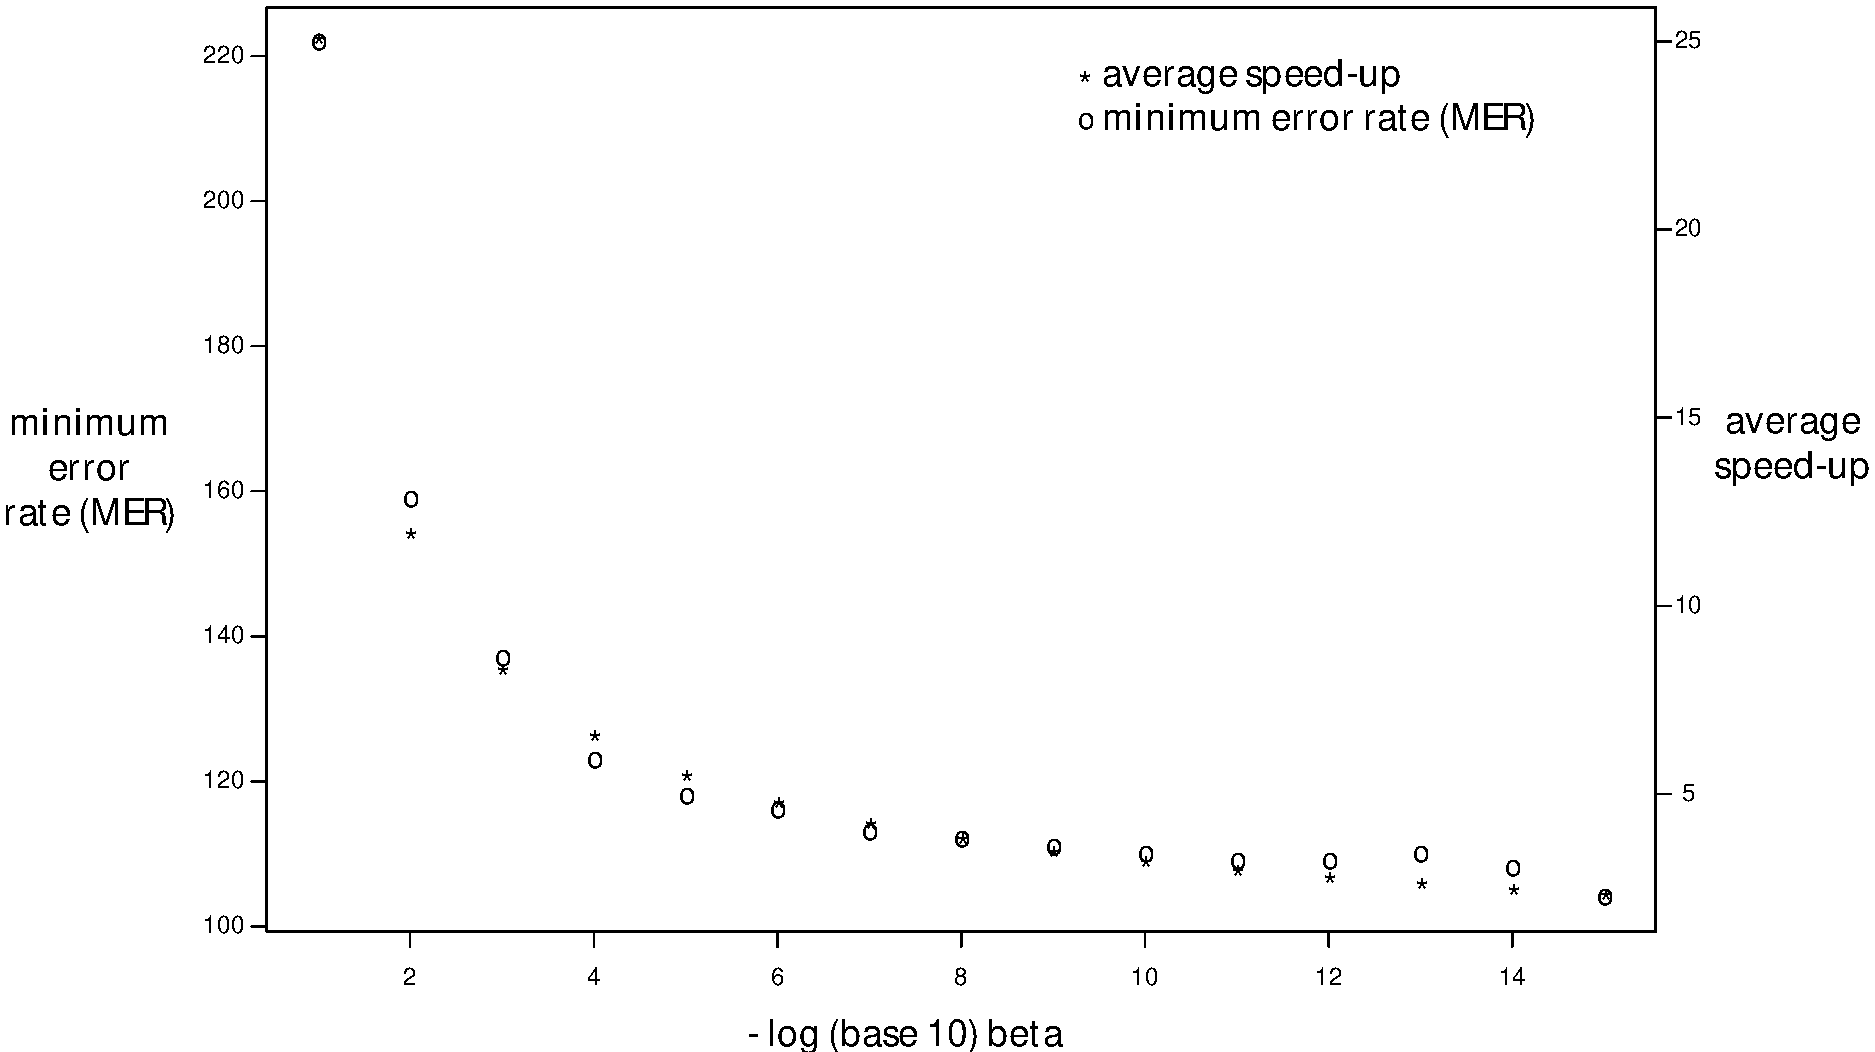
\includegraphics[width=6.4in]{figs/d5_beta_vs}
\caption{\textbf{Effect of varying the $\beta$ parameter on
    sensitivity, specificity, and speedup.}
}
\label{fig:betavaried}
\end{center}
\end{figure}

% This is \ref{fig:betavaried}
\fi

How well does QDB accelerate CM searches?  Figure~\ref{fig:speedup}
shows the time required for searching the 1 Mb benchmark target
sequence with each of the 51 models, as a function of the average
query RNA length. QDB reduces the average-case running time complexity
of the CM search algorithm from $LN^{2.36}$ to $LN^{1.32}$. Observed
accelerations relative to the standard algorithm range from 1.4-fold
(for the IRE, iron response element) to 12.7-fold (for CsrB RNA), with
an average speed-up per family of 4.2-fold. In total search time for
the benchmark (sum of all 51 searches), the acceleration is six-fold,
because large queries have disproportionate effect on the total
time.

\ifdraft
\begin{figure}
\begin{center}
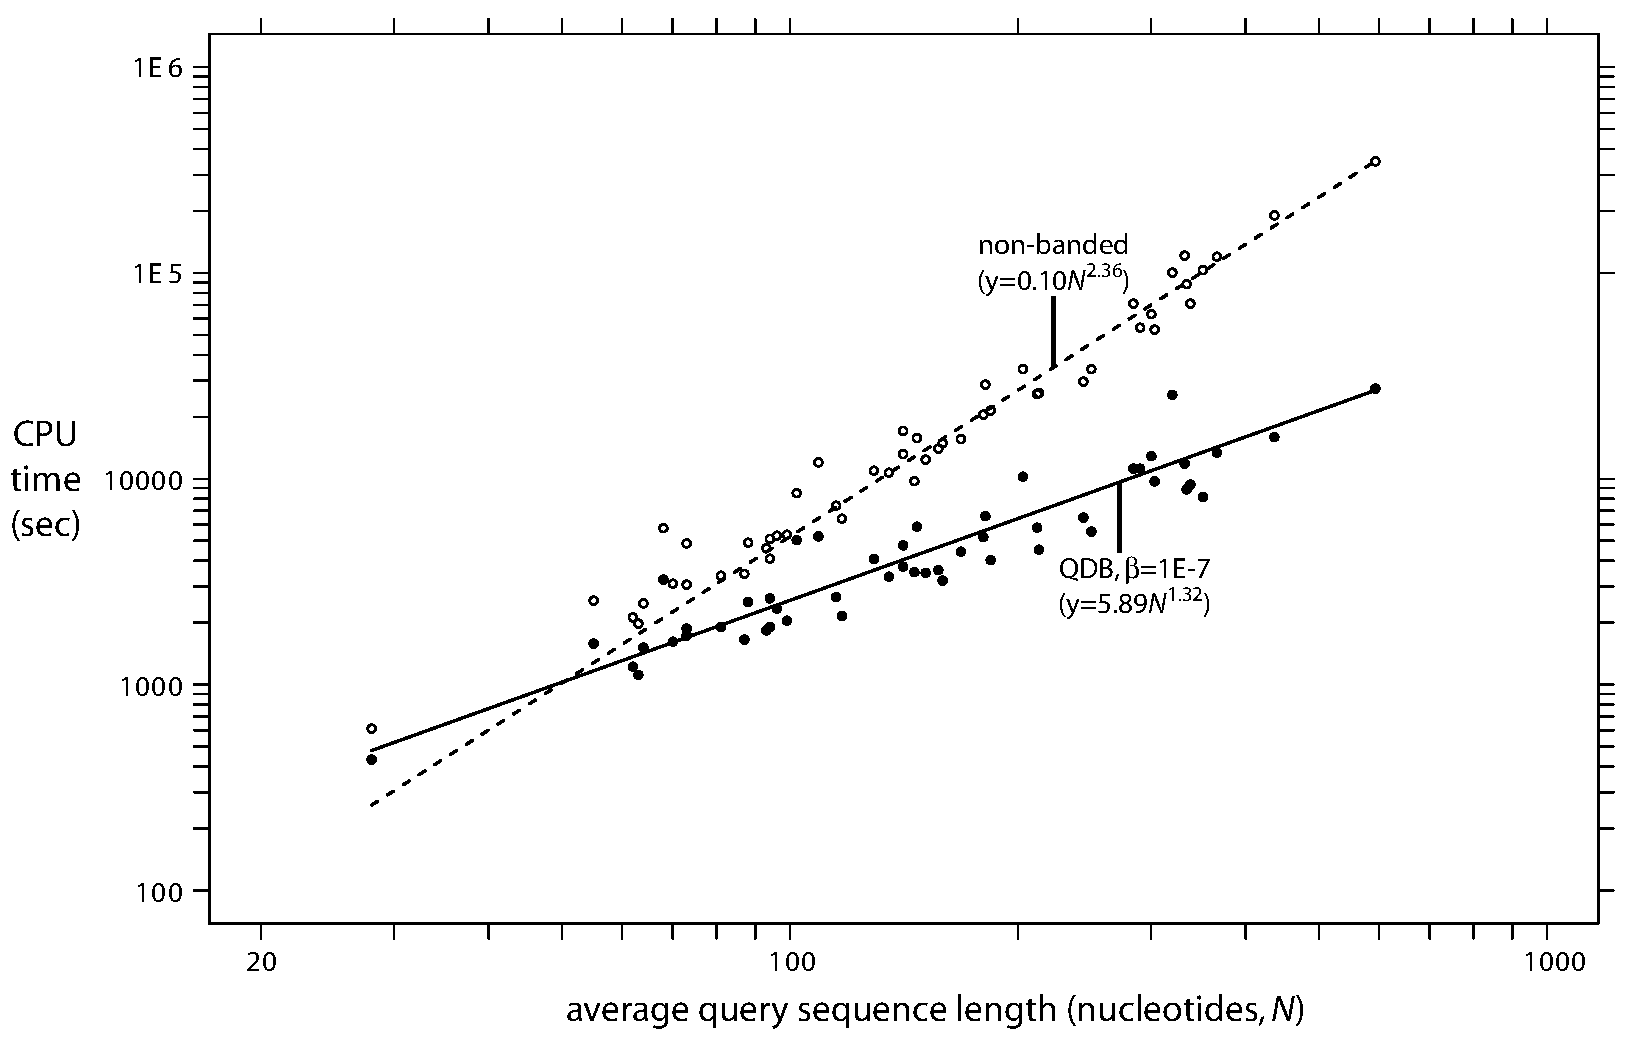
\includegraphics[width=6.4in]{figs/speedup}
\caption{\textbf{CPU time required by CM searches with and without
    QDB.} The time required for searching the 1 Mb target pseudogenome
    with each of the 51 benchmark models is shown as a point, plotted
    on a log-log graph as a function of the average length of the RNA
    sequences in the query alignment; open circles are without QDB,
    and filled circles are with QDB (with the default $\beta =
    1e-7$). Lines represent fits to a power law ($aN^b$), showing that
    for a fixed $L=$ 1 Mb target database size, the standard CYK
    algorithm empirically scales as $N^{2.36}$ and the QDB algorithm
    scales as $N^{1.32}$. The apparent intersection of the linear
    fitted lines is deceptive. At small query lengths,
    run time is dominated by factors other than the CM alignment
    computation, such as i/o. QDB searches are always faster
    than non-banded searches even for synthetic tiny
    queries of less than 10 nt (data not shown).}
\label{fig:speedup}
\end{center}
\end{figure}



% This is \ref{fig:speedup}
\fi

How much does QDB impact sensitivity and specificity? Optimal
alignments are not guaranteed to lie within QDB's high-probability
bands. This is expected to compromise sensitivity. The hope is
that QDB's bands are sufficiently wide and accurate that the loss is
negligible.  Figure~\ref{fig:roc} shows ROC plots (sensitivity versus
false positive rate) on the benchmark for the new version of
\textsc{infernal} (version 0.72) in standard versus QDB mode.  These
plots are nearly superposed, showing that the loss in accuracy is
small at the default QDB setting of $\beta=10^{-7}$.

\ifdraft
\begin{figure}
\begin{center}
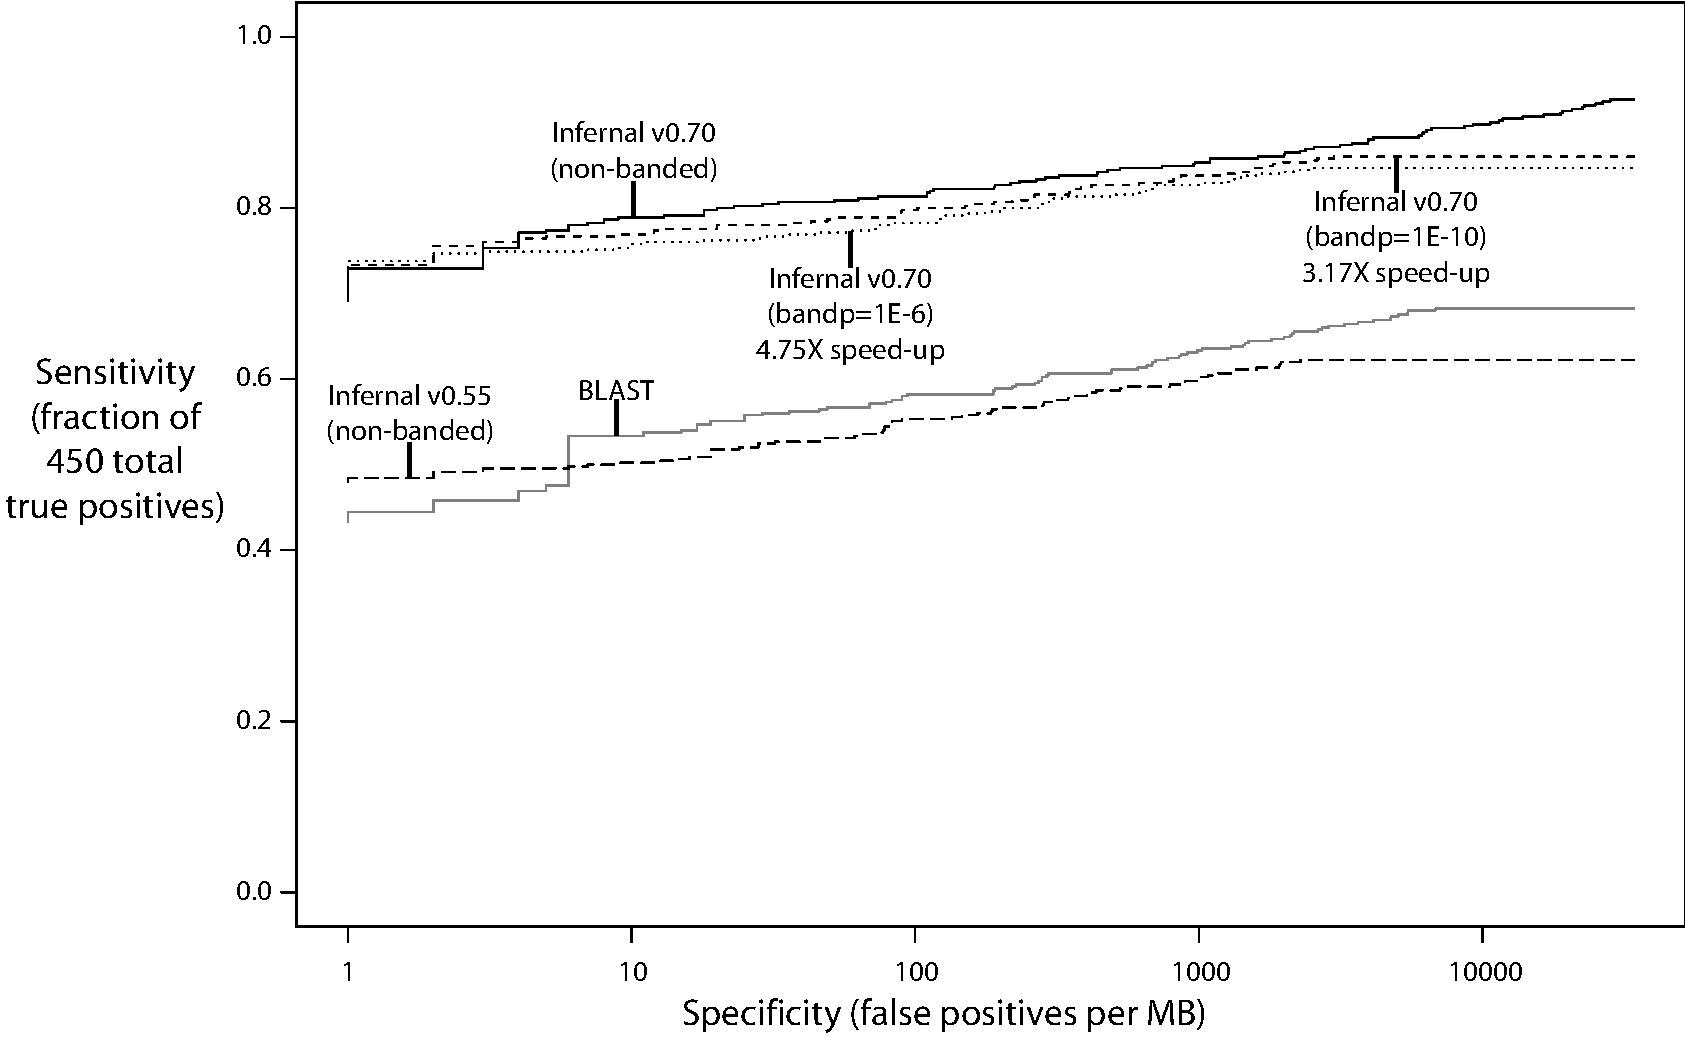
\includegraphics[width=6.4in,angle=0]{figs/d2roc_ai}
\end{center}
\caption{\textbf{ROC curves for the benchmark.}  Plots are shown for
the new \textsc{Infernal} 0.71 with and without QDB, for the old
\textsc{Infernal 0.55}, and for family-pairwise-searches with BLASTN.
}
\label{fig:roc}
\end{figure}

% This is \ref{fig:roc}
\fi

How much do our changes in parameterization (the addition of
informative Dirichlet priors and entropy weighting) improve
sensitivity and specificity? Figure~\ref{fig:roc} shows that the new
\textsc{infernal} 0.72 is a large improvement over the previous
\textsc{infernal} version 0.55, independent of QDB. (On average, in
this benchmark, \textsc{infernal} 0.55 is no better than a
family-pairwise-search with \textsc{blastn}.) Table~\ref{tbl:rmarkmerlist}
breaks this result down in more detail, showing summary and
family-specific MER scores for a variety of combinations of prior,
entropy weighting, and QDB. These results show that both informative
priors and entropy weighting individually contributed large
improvements in sensitivity and specificity.

\ifdraft
%%%%%%%%%%%%%%%%%%%%%%%%%%%%%%%%%%%%%%%%%%%%%%%%%%%%%%%%%%%%%%%%%%%%%%%
% The rmark MER table - summary MERs
%\normalfont\ttfamily
\begin{table}[htb]
\begin{center}
%\begin{tabular}{|c|c|ccc|cc|} 
\begin{tabular}{cccccc} 

%\multicolumn{1}{c}{} & \multicolumn{1}{c}{} & \multicolumn{1}{c}{} &
%\multicolumn{1}{c}{} & \multicolumn{1}{c}{} & \multicolumn{1}{c}{} &
%\multicolumn{1}{c}{summed} \\

\multicolumn{1}{c}{} & \multicolumn{1}{c}{} &
\multicolumn{1}{c}{} & \multicolumn{1}{c}{} &
\multicolumn{1}{c}{summary} & \multicolumn{1}{c}{family-specific} \\

\multicolumn{1}{c}{program} &
\multicolumn{1}{c}{prior} & \multicolumn{1}{c}{entropy (bits)} &
\multicolumn{1}{c}{$\beta$} & \multicolumn{1}{c}{MER} &
\multicolumn{1}{c}{MER} \\ \hline
\textsc{blastn}         & -           & -    & -       & 216 & 188 \\
\textsc{infernal} 0.55  & plus-1      & -    & -       & 232 & 180 \\
\textsc{infernal} 0.71  & plus-1      & -    & -       & 216 & 190 \\
\textsc{infernal} 0.71  & plus-1      & 1.46 & -       & 208 & 191 \\
%\infernal 0.71  & plus-1      & 1.46 & $1e-7$  & ? & ? \\
\textsc{infernal} 0.71  & informative & -    & -       & 179 & 163 \\
\textsc{infernal} 0.71  & informative & 1.46 & -       & 104 &  89 \\
\textsc{infernal} 0.71  & informative & 1.46 & $10^{-7}$ & 113 &  97 \\ 
%\blast-W3 & - & - & - & - & 220 & 189 & 330 & 227 & 376 & 237 \\
%\blast-W11 & - & - & - & - & 244 & 218 & 294 & 242 & 341 & 262 \\ \hline
%\infernal glocal & N & - & - & - & 275 & 229 & - & - & - & - \\
%\infernal glocal & Y & - & - & - & 253 & 215 & - & - & - & - \\
%\infernal glocal & Y & 0.54 & - & - & 155 & 104 & 80 & 53 & 69 & 28 \\
%\infernal glocal & Y & 0.54 & - & 1E-6 & 161 & 112 & - & - & - & - \\
%\infernal glocal & Y & 0.54 & - & 1E-10 & 155 & 105 & - & - & - & - \\ \hline
\end{tabular}
\end{center}
\caption{\textbf{Rfam benchmark MER summary statistics.} 
    prior: ``plus-1'' if uninformative Laplace plus-1 priors were
    used; ``informative'' if new Dirichlet priors were used.
    entropy: target model entropy in bits for entropy weighting; ``-''
    if entropy weighting was not used.
    %(effective sequence number is number of sequences in training alignment).
    %    EL: EL self transition probability used.
    ``$\beta$'': tail probability loss for banded calculation used; ``-'' if search
    was non-banded. summary MER: MER across 51 benchmark
    families; family-specific MER: MER for each family, summed
    over all 51 families. Program versions: Row 1: WU-BLASTN-2.0MP
    --kap -W=7. For \textsc{infernal} version 0.55, window length values (W)
    were preset as calculated in version 0.71 with plus-1 priors.}
\label{tbl:rmarkmerlist}
\end{table}


% This is tbl:rmarkmerlist
\fi


\section{Discussion}

\begin{comment}
%old
CM searches take a long time, and this is the most limiting factor in
using the \textsc{infernal} software to identify RNA similarities.
Prior to this work, \textsc{infernal} (version 0.55) required 508
CPU-hours to search 51 models against just 1 megabase of sequence in
our benchmarks (Table~\ref{tbl:rmark}). With QDB (version 0.72), this
time is reduced to 84.51 hours, a six-fold speed-up. Our eventual goal
is to enable routine genome annotation of structural RNAs: to be able
to search thousands of RNA models against complete genome sequences.
A search of all 503 Rfam 7.0 models against the 3 GB human genome
would take on the order of 2000 CPU-years. We need to be able to do it
in at most a few days, so we need to increase CM search speed by five
to six orders of magnitude. Parallelization is feasible, but even
large clusters will give us only about three orders of magnitude.
Moreover, parallelization on this scale is prohibitively expensive for
all but a few centers. Software improvement (code optimization) will
contribute, but probably only about two-fold.  Hardware improvements
will contribute about two-fold per year or so so long as Moore's law
continues. None of this is sufficient for our immediate purposes.
Algorithmic acceleration is demanded.

The QDB algorithm is a partial but not a complete solution to the
problem. At $\beta$ banding cutoffs that do not appreciably compromise
sensitivity and specificity, QDB offers about a six-fold
speedup in CM searches. However, QDB combines synergistically with
parallelization, code optimization, and hardware improvements, as well
as with the filtering methods recently described by Weinberg and Ruzzo
\cite{WeinbergRuzzo04,WeinbergRuzzo04b,WeinbergRuzzo06}, so we view QDB as part of a
growing suite of approaches that we can combine to accelerate
\textsc{infernal}.
\end{comment}

%new
CM searches take a long time, and this is the most limiting factor in
using the \textsc{infernal} software to identify RNA similarities.
Prior to this work, \textsc{infernal} 0.55 required 508 CPU-hours to
search 51 models against just 1 megabase of sequence in our benchmarks
(Table~\ref{tbl:rmark}).  Using QDB with $\beta$ banding cutoffs that
do not appreciably compromise sensitivity and specificity,
\textsc{infernal} 0.72 offers a six-fold speedup, performing the
benchmark in 85 hours.  Our eventual goal is to enable routine genome
annotation of structural RNAs: to be able to search thousands of RNA
models against complete genome sequences.  A search of all 503 Rfam
7.0 models against the 3 GB human genome with \textsc{infernal} 0.72
in QDB mode would take on the order of 300 CPU-years (down from 1800
with \textsc{infernal} 0.55).  We need to be able to do it in at most
a few days, so we still need to increase CM search speed by five
orders of magnitude.  Thus, the QDB algorithm is a partial but
certainly not complete solution to the problem. However, QDB combines
synergistically with other acceleration techniques. Parallelization,
on large clusters (though prohibitively expensive for all but a few
centers) could give us further acceleration of three orders of
magnitude.  Software improvement (code optimization) will also
contribute, but probably only about two-fold.  Hardware improvements
will contribute about two-fold per year or so so long as Moore's law
continues. Finally, QDB is complementary to the filtering methods
recently described by Weinberg and Ruzzo
\cite{WeinbergRuzzo04,WeinbergRuzzo04b,WeinbergRuzzo06}. We view QDB
as part of a growing suite of approaches that we can combine to
accelerate \textsc{infernal}.

Is it really worth burning all this CPU time in the first place?  Do
CM searches identify structural RNA homologies that other methods
miss? Obviously we think so, but one would like to see convincing
results. For large, diverse RNA families like tRNA, where a CM can be
trained on over a thousand well-aligned sequences with a
well-conserved consensus secondary structure, CM approaches have been
quite powerful. The state of the art in large scale tRNA gene
identification remains the CM-based program \textsc{trnascan-se}
\cite{LoweEddy97}, and CMs were also used, for example, to discover
the divergent tRNA for pyrrolysine, the ``22nd amino acid''
\cite{Srinivasan02}. But Figure~\ref{fig:roc} shows that on average,
over 51 more or less ``typical'' RNA families of various sizes and
alignment quality, \textsc{infernal} 0.55 was actually no better than
doing a family-pairwise-search with \textsc{blastn}.  Until recently,
we have spent relatively little effort on how \textsc{infernal}
parameterizes its models, and relatively more on reducing its
computational requirements \cite{Eddy02b}, so previous versions of
\textsc{infernal} have performed best where naive parameterization
works best: on very large, high-quality alignments of hundreds of
sequences, which are atypical of many interesting homology search
problems.

In this work, partly because the level of acceleration achieved by QDB
is sensitive to transition parameterization, we have brought
\textsc{infernal} parameterization close to the state of the art in
profile HMMs, by introducing mixture Dirichlet priors
\cite{Sjolander96} and entropy weighting \cite{Karplus98}. This
resulted in a large improvement in the sensitivity and specificity of
searches, as judged by our benchmark (Figure~\ref{fig:roc}). The
difference between \textsc{infernal} and family-pairwise
\textsc{blastn} now appears pronounced for average-case behavior, not
just best-case behavior. However, while we trust our benchmarking to
tell us we have greatly improved \textsc{infernal} relative to
previous versions of itself, our benchmarking does not allow us to
draw firm conclusions about our performance relative to other
software. For that, we prefer to see independent
benchmarks. Benchmarks by tool developers are notoriously biased, and
however honest we may try to be, some biases are essentially
unavoidable. For one thing, establishing an internal benchmark for
ongoing code development creates an insidious form of training on the
test set, because we accept code changes that improve benchmark
performance.  In particular, we set the entropy weighting target of
1.46 bits and the numbers of mixture prior components by optimizing
against our benchmark.  Further, our benchmark does not use a
realistic model for the background sequence of the ``pseudo-genome'',
because we construct the background as a homogeneous IID (independent,
identically distributed) sequence, and this poorly reflects the
heterogeneous and repetitive nature of genomic sequence.  This
benchmark should be sufficient for an internal comparison of versions
0.55 and 0.72 of \textsc{infernal}, because we have not altered how
\textsc{infernal} deals with heterogeneous compositional bias. But we
cannot safely draw conclusions from our simple benchmark about the
relative performance of \textsc{infernal} and \textsc{blast} on real
searches, for example, because \textsc{blast} may (and in fact does)
treat sequence heterogeneity better than \textsc{infernal} does.  In
this regard, currently we are aware of only one independent benchmark
BRaliBase III \cite{Freyhult07}. BRaliBase III consists of many
different query alignments of 5 or 20 RNA sequences, drawn from three
different RNA families (U5, 5S rRNA, and tRNA). These authors' results
broadly confirm our internal observations: while \textsc{infernal}
0.55 showed mediocre performance compared to \textsc{blastn} and
several other tools, a recent version of \textsc{infernal} stood out
as a superior method for RNA similarity search.

Nonetheless, though \textsc{infernal} 0.72 shows large improvements in
speed, sensitivity, and specificity over previous versions, there are
numerous areas where we need to improve further. 

A significant gap in our current implementation is that
\textsc{infernal} reports only raw bit scores, and does not yet report
expectation values (E-values). CM local alignment scores empirically
follow a Gumbel (extreme value) distribution \cite{KleinEddy03}, just
as local sequence alignment scores do \cite{KarlinAltschul93}, so
there are no technical hurdles in implementing E-values. This will be
an immediate focus for the next version of \textsc{infernal}.  E-value
calculations not only have the effect of reporting statistical
significance (more meaningful to a user than a raw bit score), but
they also normalize each family's score distribution into a more
consistent overall rank order, because different query models exhibit
different null distributions (particularly in the location parameter
of the Gumbel distribution). We therefore expect E-values to
contribute a large increase in performance whenever a single
family-independent threshold is set. Table~\ref{tbl:rmarkmerlist}
roughly illustrates the expected gain, by showing the large difference
between summary MER scores and family-specific MER scores.

Parameterization of both CMs and profile HMMs remains problematic,
because these methods continue to assume that training sequences are
statistically independent, when in fact they are related (often
strongly so) by phylogeny. Methods like sequence weighting and entropy
weighting do help, but they are \emph{ad hoc} hacks: unsatisfying and
unlikely to be optimal. Even mixture Dirichlet priors, though they
appear to be mathematically sophisticated, fundamentally assume that
observed counts are drawn as independent multinomial samples, and
therefore the use of Dirichlet priors is fundamentally flawed.
Probabilistic phylogenetic inference methodology needs to be
integrated with profile search methods. This is an area of active
research \cite{Holmes04, Holmes05b, Rivas05} in which important
challenges remain, particularly in the treatment of insertions and
deletions.

Finally, QDB is not the only algorithmic acceleration method we can
envision.  Michael Brown described a complementary banding method to
accelerate his SCFG-based \textsc{rnacad} ribosomal RNA alignment
software \cite{Brown00}, in which he uses profile HMM based sequence
alignment to the target to determine bands where the more rigorous
SCFG-based alignment should fall (because some regions of the
alignment are well-determined based solely on sequence alignment). The
gapped \textsc{blast} algorithm (seed word hits, ungapped hit extension, and
banded dynamic programming) can conceivably be extended from
two-dimensional sequence alignment to three-dimensional CM dynamic
programming lattices. Developing such algorithms -- and incorporating
them into a widely useful, freely available codebase -- are priorities
for us.

\section{Materials and Methods}

The version and options used for \textsc{blast} in our benchmark are
\texttt{WU-BLASTN-2.0MP --kap -W=7}.  For \textsc{infernal}, versions 0.55
and 0.72 were used as indicated. The complete \textsc{infernal}
software package, including documentation and the Rfam-based benchmark
described here, may be downloaded from
\url{http://infernal.janelia.org}. It is developed on GNU/Linux
operating systems but should be portable to any POSIX-compliant
operating system, including Mac OS/X. It is freely licensed under the
GNU General Public License.

The ANSI C code we used for estimating maximum likelihood mixture
Dirichlet priors depends on a copyrighted and nonredistributable
implementation of the conjugate gradient descent algorithm from
Numerical Recipes in C \cite{Press93}. Our code, less the Numerical
Recipes routine, is freely available upon request.


\section{Acknowledgements}
We thank Elena Rivas for critical comments on the manuscript.

\section{Funding}
EPN gratefully acknowledges financial support from an NIH NHGRI
Institutional Training Grant in Genomic Science, T32-HG000045. Work in
SRE's lab in Washington University in St. Louis, where this work was
initiated, was supported by NIH NHGRI RO1-HG01363, HHMI, and Alvin
Goldfarb. 

\newpage
%\bibliography{distilled}
\bibliography{master,books,lab}

\ifdraft
 \relax
\else

\newpage
\renewcommand{\baselinestretch}{1.0}
\begin{table}
\renewcommand{\tabcolsep}{0.7em}
\tiny
\begin{center}
%\begin{tabular}{|r|r|l|l|l||l|r||l|r||l|r||l|r||l|r||l|r||} \hline
\begin{tabular}{|rr|rr|cc|c|c|cc|cc|cc|cc|cc|cc|} \cline{1-6} \cline{8-20}
%\multicolumn{5}{c}{} & \multicolumn{2}{|c|}{1} & \multicolumn{2}{|c|}{2} & \multicolumn{2}{|c|}{3} & \multicolumn{2}{|c|}{4} & \multicolumn{2}{|c|}{5} & \multicolumn{2}{|c|}{6} \\ \cline{1-17}
\multicolumn{1}{|c}{dist} & \multicolumn{1}{c|}{tied} &
  \multicolumn{1}{c}{dist} & \multicolumn{1}{c|}{grp} & node & next &
  & \multicolumn{13}{|c|}{Dirichlet $\alpha$ parameters} \\ %\cline{8-20}
%\multicolumn{1}{|c}{\#} & \multicolumn{1}{c|}{\#} & \multicolumn{1}{c}{counts} & \multicolumn{1}{c|}{counts} & state & node & & $|\alpha|$ & $a_1$ &
%  $\frac{\alpha_{a_1}}{|\alpha|}$ & $a_2$ & $\frac{\alpha_{a_2}}{|\alpha|}$ & $a_3$ &
%  $\frac{\alpha_{a_3}}{|\alpha|}$ & $a_4$ & $\frac{\alpha_{a_4}}{|\alpha|}$ & $a_5$ &
%  $\frac{\alpha_{a_5}}{|\alpha|}$ & $a_6$ & $\frac{\alpha_{a_6}}{|\alpha|}$ \\
%  \cline{1-6} \cline {8-20} 
\multicolumn{1}{|c}{\#} & \multicolumn{1}{c|}{to} & \multicolumn{1}{c}{counts} & \multicolumn{1}{c|}{counts} & state & node & & $|\alpha|$ & $a$ &
  $\frac{\alpha_{a}}{|\alpha|}$ & $a$ & $\frac{\alpha_{a}}{|\alpha|}$ & $a$ &
  $\frac{\alpha_{a}}{|\alpha|}$ & $a$ & $\frac{\alpha_{a}}{|\alpha|}$ & $a$ &
  $\frac{\alpha_{a}}{|\alpha|}$ & $a$ & $\frac{\alpha_{a}}{|\alpha|}$ \\
  \cline{1-6} \cline {8-20} 

1   &    & 6     & 11    & MATP\_MP & BIF  & & 0.5509  & IL & 0.1229 & IR & 0.0001 & B  & 0.8770 &    &        &    &  &  &  \\  
2   &    & 7023  & 7119  & MATP\_MP & MATP & & 7.2986  & IL & 0.0023 & IR & 0.0024 & MP & 0.9816 & ML & 0.0056 & MR & 0.0046 & D & 0.0035 \\  
3   &    & 1600  & 1830  & MATP\_MP & MATL & & 1.5914  & IL & 0.0179 & IR & 0.0155 & ML & 0.9200 & D  & 0.0466 &    &  &  &  \\  
4   &    & 145   & 195   & MATP\_MP & MATR & & 1.9038  & IL & 0.0173 & IR & 0.0073 & MR & 0.8903 & D  & 0.0852 &    &  &  &  \\  
5   & 1  & 2     & 11    & MATP\_MP & END  & & 0.5509  & IL & 0.1229 & IR & 0.0001 & E  & 0.8770 &    &        &    &  &  &  \\  
6*  &    & 1     & 2     & MATP\_ML & BIF  & & 3.0000  & IL & 0.3333 & IR & 0.3333 & B  & 0.3333 &    &        &    &  &  &  \\  
7   &    & 577   & 577   & MATP\_ML & MATP & & 0.6941  & IL & 0.0131 & IR & 0.0103 & MP & 0.4032 & ML & 0.4983 & MR & 0.0115 & D & 0.0636 \\  
8   &    & 133   & 133   & MATP\_ML & MATL & & 0.9316  & IL & 0.0739 & IR & 0.0651 & ML & 0.7038 & D  & 0.1571 &    &  &  &  \\  
9   &    & 15    & 15    & MATP\_ML & MATR & & 0.3272  & IL & 0.1884 & IR & 0.0432 & MR & 0.4082 & D  & 0.3602 &    &  &  &  \\  
10* & 6  & 1     & 2     & MATP\_ML & END  & & 3.0000  & IL & 0.3333 & IR & 0.3333 & E  & 0.3333 &    &        &    &  &  &  \\  
11* &    & 1     & 2     & MATP\_MR & BIF  & & 3.0000  & IL & 0.3333 & IR & 0.3333 & B  & 0.3333 &    &        &    &  &  &  \\  
12  &    & 531   & 531   & MATP\_MR & MATP & & 0.7987  & IL & 0.0079 & IR & 0.0190 & MP & 0.3241 & ML & 0.0193 & MR & 0.5631 & D & 0.0666 \\  
13  &    & 151   & 151   & MATP\_MR & MATL & & 0.6933  & IL & 0.0357 & IR & 0.0699 & ML & 0.3066 & D  & 0.5879 &    &  &  &  \\  
14  &    & 15    & 15    & MATP\_MR & MATR & & 0.3574  & IL & 0.0582 & IR & 0.0002 & MR & 0.7629 & D  & 0.1787 &    &  &  &  \\  
15* & 11 & 1     & 2     & MATP\_MR & END  & & 3.0000  & IL & 0.3333 & IR & 0.3333 & E  & 0.3333 &    &        &    &  &  &  \\  
16* &    & 0     & 2     & MATP\_D  & BIF  & & 3.0000  & IL & 0.3333 & IR & 0.3333 & B  & 0.3333 &    &        &    &  &  &  \\  
17  &    & 575   & 575   & MATP\_D  & MATP & & 0.5450  & IL & 0.0019 & IR & 0.0047 & MP & 0.0857 & ML & 0.0534 & MR & 0.0528 & D & 0.8015 \\  
18  &    & 149   & 149   & MATP\_D  & MATL & & 0.5831  & IL & 0.0421 & IR & 0.0526 & ML & 0.2080 & D  & 0.6973 &    &  &  &  \\  
19  &    & 14    & 14    & MATP\_D  & MATR & & 0.1164  & IL & 0.0001 & IR & 0.0001 & MR & 0.2439 & D  & 0.7559 &    &  &  &  \\  
20* & 16 & 2     & 2     & MATP\_D  & END  & & 3.0000  & IL & 0.3333 & IR & 0.3333 & E  & 0.3333 &    &        &    &  &  &  \\  
21  &    & 2     & 4     & MATP\_IL & BIF  & & 1.4397  & IL & 0.6553 & IR & 0.0445 & B  & 0.3002 &    &        &    &  &  &  \\  
22  &    & 121   & 126   & MATP\_IL & MATP & & 0.9402  & IL & 0.1673 & IR & 0.1394 & MP & 0.5904 & ML & 0.0443 & MR & 0.0259 & D & 0.0327 \\  
23  &    & 114   & 119   & MATP\_IL & MATL & & 0.8046  & IL & 0.3108 & IR & 0.1936 & ML & 0.4610 & D  & 0.0346 &    &  &  &  \\  
24  &    & 14    & 15    & MATP\_IL & MATR & & 1.0926  & IL & 0.1419 & IR & 0.0501 & MR & 0.6538 & D  & 0.1541 &    &  &  &  \\  
25  & 21 & 2     & 4     & MATP\_IL & END  & & 1.4397  & IL & 0.6553 & IR & 0.0445 & E  & 0.3002 &    &        &    &  &  &  \\  
26  &    & 1     & 31    & MATP\_IR & BIF  & & 0.9361  & IR & 0.2827 & B  & 0.7173 &    &        &    &        &    &  &  &  \\  
27  &    & 145   & 227   & MATP\_IR & MATP & & 1.5494  & IR & 0.1884 & MP & 0.7090 & ML & 0.0165 & MR & 0.0588 & D  & 0.0273 &  &  \\  
28  &    & 129   & 701   & MATP\_IR & MATL & & 1.6332  & IR & 0.3681 & ML & 0.5752 & D  & 0.0566 &    &        &    &  &  &  \\  
29  &    & 8     & 160   & MATP\_IR & MATR & & 1.2428  & IR & 0.2633 & MR & 0.6809 & D  & 0.0558 &    &        &    &  &  &  \\  
30  & 26 & 0     & 31    & MATP\_IR & END  & & 0.9361  & IR & 0.2827 & E  & 0.7173 &    &        &    &        &    &  &  &  \\  
31  &    & 108   & 1130  & MATL\_ML & BIF  & & 1.2298  & IL & 0.0078 & B  & 0.9922 &    &        &    &        &    &  &  &  \\  
32  &    & 420   & 1319  & MATL\_ML & MATP & & 2.4162  & IL & 0.0132 & MP & 0.9520 & ML & 0.0150 & MR & 0.0129 & D  & 0.0070 &  &  \\  
33  &    & 19013 & 19371 & MATL\_ML & MATL & & 1.8632  & IL & 0.0082 & ML & 0.9711 & D  & 0.0207 &    &        &    &  &  &  \\  
34  &    & 859   & 6692  & MATL\_ML & MATR & & 72.1283 & IL & 0.0058 & MR & 0.9755 & D  & 0.0187 &    &        &    &  &  &  \\  
35  & 31 & 801   & 1130  & MATL\_ML & END  & & 1.2298  & IL & 0.0078 & E  & 0.9922 &    &        &    &        &    &  &  &  \\  
36  &    & 28    & 172   & MATL\_D  & BIF  & & 6.8008  & IL & 0.0029 & B  & 0.9971 &    &        &    &        &    &  &  &  \\  
37  &    & 103   & 103   & MATL\_D  & MATP & & 0.7288  & IL & 0.0321 & MP & 0.5730 & ML & 0.0536 & MR & 0.1654 & D  & 0.1758 &  &  \\  
38  &    & 3152  & 3152  & MATL\_D  & MATL & & 0.4101  & IL & 0.0138 & ML & 0.3105 & D  & 0.6756 &    &        &    &  &  &  \\  
39  &    & 154   & 154   & MATL\_D  & MATR & & 0.6736  & IL & 0.0203 & MR & 0.6014 & D  & 0.3782 &    &        &    &  &  &  \\  
40  & 36 & 144   & 172   & MATL\_D  & END  & & 6.8008  & IL & 0.0029 & E  & 0.9971 &    &        &    &        &    &  &  &  \\  
41  & 26 & 13    & 31    & MATL\_IL & BIF  & & 0.9361  & IL & 0.2827 & B  & 0.7173 &    &        &    &        &    &  &  &  \\  
42  & 27 & 35    & 227   & MATL\_IL & MATP & & 1.5494  & IL & 0.1884 & MP & 0.7090 & ML & 0.0588 & MR & 0.0165 & D  & 0.0273 &  &  \\  
43  & 28 & 549   & 701   & MATL\_IL & MATL & & 1.6332  & IL & 0.3681 & ML & 0.5752 & D  & 0.0566 &    &        &    &  &  &  \\  
44  & 29 & 45    & 160   & MATL\_IL & MATR & & 1.2428  & IL & 0.2633 & MR & 0.6809 & D  & 0.0558 &    &        &    &  &  &  \\  
45  & 26 & 0     & 31    & MATL\_IL & END  & & 0.9361  & IL & 0.2827 & E  & 0.7173 &    &        &    &        &    &  &  &  \\  
46  & 31 & 206   & 1130  & MATR\_MR & BIF  & & 1.2298  & IR & 0.0078 & B  & 0.9922 &    &        &    &        &    &  &  &  \\  
47  & 32 & 848   & 1319  & MATR\_MR & MATP & & 2.4162  & IR & 0.0132 & MP & 0.9520 & ML & 0.0150 & MR & 0.0129 & D  & 0.0070 &  &  \\  
48  & 34 & 5833  & 6692  & MATR\_MR & MATR & & 2.1283  & IR & 0.0058 & MR & 0.9755 & D  & 0.0187 &    &        &    &  &  &  \\  
49  &    & 39    & 39    & MATR\_D  & BIF  & & 0.4664  & IR & 0.0463 & B  & 0.9537 &    &        &    &        &    &  &  &  \\  
50  &    & 176   & 176   & MATR\_D  & MATP & & 0.8689  & IR & 0.0245 & MP & 0.6126 & ML & 0.1269 & MR & 0.0471 & D  & 0.1890 &  &  \\  
51  &    & 771   & 771   & MATR\_D  & MATR & & 0.4869  & IR & 0.0119 & MR & 0.3373 & D  & 0.6507 &    &        &    &  &  &  \\  
52  & 26 & 15    & 31    & MATR\_IR & BIF  & & 0.9361  & IR & 0.2827 & B  & 0.7173 &    &        &    &        &    &   &  &  \\  
53  & 27 & 39    & 227   & MATR\_IR & MATP & & 1.5494  & IR & 0.1884 & MP & 0.7090 & ML & 0.0165 & MR & 0.0588 & D  & 0.0273 &  &  \\  
54  & 29 & 107   & 160   & MATR\_IR & MATR & & 1.2428  & IR & 0.2633 & MR & 0.6809 & D  & 0.0558 &    &        &    &  &  &  \\  
%55 &    &       &       & BEGL\_S  & BIF  & & 1.0000  & B  & 1.0000 &    &        &    &        &    &        &    &  &  &  \\  
55  &    & 338   & 338   & BEGL\_S  & MATP & & 5.0422  & MP & 0.9579 & ML & 0.0121 & MR & 0.0183 & D  & 0.0117 &    &   &  &  \\  
56  & 31 & 15    & 1130  & BEGR\_S  & BIF  & & 1.2298  & IL & 0.0078 & B  & 0.9922 &    &        &    &        &    &  &  &  \\  
57  & 32 & 51    & 1319  & BEGR\_S  & MATP & & 2.4162  & IL & 0.0132 & MP & 0.9520 & ML & 0.0150 & MR & 0.0129 & D  & 0.0070 &  &  \\  
58  & 33 & 358   & 19371 & BEGR\_S  & MATL & & 1.8632  & IL & 0.0082 & ML & 0.9711 & D  & 0.0207 &    &        &    &  &  &  \\  
59  & 26 & 2     & 31    & BEGR\_IL & BIF  & & 0.9361  & IL & 0.2827 & B  & 0.7173 &    &        &    &        &    &   &  &  \\  
60  & 27 & 3     & 227   & BEGR\_IL & MATP & & 1.5494  & IL & 0.1884 & MP & 0.7090 & ML & 0.0588 & MR & 0.0165 & D  & 0.0273 &  &  \\  
61  & 28 & 19    & 701   & BEGR\_IL & MATL & & 1.6332  & IL & 0.3681 & ML & 0.5752 & D  & 0.0566 &    &        &    &  &  &  \\  
62  & 1  & 3     & 11    & ROOT\_S  & BIF  & & 0.5509  & IL & 0.1229 & IR & 0.0001 & B  & 0.8770 &    &        &    &  &  &  \\  
63  & 2  & 96    & 7119  & ROOT\_S  & MATP & & 7.2986  & IL & 0.0023 & IR & 0.0024 & MP & 0.9816 & ML & 0.0056 & MR & 0.0046 & D & 0.0035 \\  
64  & 3  & 230   & 1830  & ROOT\_S  & MATL & & 1.5914  & IL & 0.0179 & IR & 0.0155 & ML & 0.9200 & D  & 0.0466 &    &  &  &  \\  
65  & 4  & 50    & 195   & ROOT\_S  & MATR & & 1.9038  & IL & 0.0173 & IR & 0.0073 & MR & 0.8903 & D  & 0.0852 &    &  &  &  \\  
66  & 21 & 0     & 4     & ROOT\_IL & BIF  & & 1.4397  & IL & 0.6553 & IR & 0.0445 & B  & 0.3002 &    &        &    &  &  &  \\  
67  & 22 & 5     & 126   & ROOT\_IL & MATP & & 0.9402  & IL & 0.1673 & IR & 0.1394 & MP & 0.5904 & ML & 0.0443 & MR & 0.0259 & D & 0.0327 \\  
68  & 23 & 5     & 119   & ROOT\_IL & MATL & & 0.8046  & IL & 0.3108 & IR & 0.1936 & ML & 0.4610 & D  & 0.0346 &    &  &  &  \\  
69  & 24 & 1     & 15    & ROOT\_IL & MATR & & 1.0926  & IL & 0.1419 & IR & 0.0501 & MR & 0.6538 & D  & 0.1541 &    &  &  &  \\  
70  & 26 & 0     & 31    & ROOT\_IR & BIF  & & 0.9361  & IR & 0.2827 & B  & 0.7173 &    &        &    &        &    &  &  &  \\  
71  & 27 & 5     & 227   & ROOT\_IR & MATP & & 1.5494  & IR & 0.1884 & MP & 0.7090 & ML & 0.0165 & MR & 0.0588 & D  & 0.0273 &  &  \\  
72  & 28 & 4     & 701   & ROOT\_IR & MATL & & 1.6332  & IR & 0.3681 & ML & 0.5752 & D  & 0.0566 &    &        &    &  &  &  \\  
73  & 29 & 0     & 160   & ROOT\_IR & MATR & & 1.2428  & IR & 0.2633 & MR & 0.6809 & D  & 0.0558 &    &        &    &  &  &  \\   \cline{1-6} \cline {8-20} 
\end{tabular}
\end{center}

\normalfont\rmfamily
\caption{\textbf{Dirichlet priors for transitions.}  ``dist \#''=
  index for the 73 different types of transition distributions in CMs;
  asterisks mark six distributions which had very few observed counts
  even after tying into groups, and for which we assigned a uniform
  plus-one Laplace prior. ``tied to''= if an index is shown in this
  column, this distribution was estimated in a group (pooling observed
  counts) with the indicated distribution.  ``dist counts''= total
  counts observed for this distribution in the training data, before
  pooling into groups. ``grp counts''= total counts for a group of one
  or more pooled distributions; this is the size of the training data
  sets for 36 different single-component Dirichlet priors.  ``node
  state''= unique CM state type the transition is from. 
  ``next node''= the node type that the transitions are going to.
  The codes for node types and state types in a CM are more fully
  explained in \cite{Eddy02b}.
}
\label{tbl:transitions}
\end{table}
\renewcommand{\baselinestretch}{1.5}


\newpage
%%%%%%%%%%%%%%%%%%%%%%%%%%%%%%%%%%%%%%%%%%%%%%%%%%%%%%%%%%%%%%%%%%%%%%%
% The emission prior alignment counts
% this table is in my rotation lab presentation ./emit_priors_revisited/nawrocki_dirichlet.pdf
%\renewcommand{\baselinestretch}{1.0}
\begin{table}
%\normalfont\ttfamily
\begin{center}
\begin{tabular}{lrrrrrrr} 
& & \# filtered & \# aln & \# consensus & \# consensus & base pair & SS \\
alignment & \# seqs & seqs & columns & base pairs  & SS columns & counts & counts \\ \hline
LSU      & 1551  & 139  & 7270 & 601 & 1532  & 65229 & 180558  \\
SSU bap  & 12773 & 254  & 2653 & 421 & 680   & 97834 & 153565  \\
SSU euk  & 7151  & 207  & 4558 & 407 & 959   & 72521 & 174260  \\
SSU mito & 1039  & 107  & 3791 & 216 & 524   & 19803 & 56510   \\ 
%\multicolumn{8}{l}{bap: contains bacterial, archaeal and plastid
%  sequences} \\
\end{tabular}
\end{center}
\caption{\textbf{Summary statistics for the dataset used for emission prior
    estimation.} ``SS'' = single-stranded.} 
\label{tbl:emissioncounts}
\end{table}


\newpage
%%%%%%%%%%%%%%%%%%%%%%%%%%%%%%%%%%%%%%%%%%%%%%%%%%%%%%%%%%%%%%%%%%%%%%%
% 04.10.06 The priors tables.
% these were sequestered to the supplementary material in draft 2,
% but they're back to the main document for draft 3.
%
% These tables were generated by dchlet2latex_d3.pl revision 369, in 
% in ~nawrocki/notebook/6_0404_inf_banded_mscript_d3/latex/dchlet_tbls_dir/:
%
% $ perl dchlet2latex_d3.pl dchlet56.prior 041006
% generates 041006_bp_priors.tex, 041006_sing_priors.tex and
%           041006_trans_priors.tex, which include the following
%           three tables (in slightly different format, I tweaked
%           them to get these).
%%%%%%%%%%%%%%%%%%%%%%%%%%%%%%%%%%%%%%%%%%%%%%%%%%%%%%%%%%%%%%%%%%%%%%%
% Base pair emission priors. 041006_bp_priors.tex (with modifications)

\begin{table}
%\normalfont\ttfamily
\footnotesize
\begin{center}
\begin{tabular}{|c|c|c|c|c|c|c|c|c|c|c|} \hline
\multicolumn{2}{|c|}{component $i$} & 1 & 2 & 3 & 4 & 5 & 6 & 7 & 8 & 9 \\
\multicolumn{2}{|c|}{$q_i$} & 0.0305 & 0.0703 & 0.1185 & 0.1810 & 0.1888 & 0.1576 & 0.0417 & 0.0959 & 0.1156 \\
\multicolumn{2}{|c|}{$|\alpha|$} & 14.3744 & 2.9920 & 26.2757 & 0.5342 &
4.2716 & 13.3232 & 33.8619 & 22.2258 & 33.1991 \\ \hline 
\multicolumn{11}{c}{} \\ \hline

$ab$ & mean $\alpha$ & $\frac{\alpha_{ab}}{|\alpha|}$ & $\frac{\alpha_{ab}}{|\alpha|}$ & $\frac{\alpha_{ab}}{|\alpha|}$ & $\frac{\alpha_{ab}}{|\alpha|}$ & $\frac{\alpha_{ab}}{|\alpha|}$ & $\frac{\alpha_{ab}}{|\alpha|}$ & $\frac{\alpha_{ab}}{|\alpha|}$ & $\frac{\alpha_{ab}}{|\alpha|}$ & $\frac{\alpha_{ab}}{|\alpha|}$ \\ \hline 
AA & 0.0063 & 0.0398 & 0.0390 & 0.0011 & 0.0017 & 0.0005 & 0.0062 & 0.0064 & 0.0058 & 0.0002 \\  
AC & 0.0092 & 0.0421 & 0.0176 & 0.0009 & 0.0152 & 0.0018 & 0.0125 & 0.0115 & 0.0051 & 0.0046 \\  
AG & 0.0052 & 0.0381 & 0.0226 & 0.0046 & 0.0034 & 0.0008 & 0.0032 & 0.0040 & 0.0053 & 0.0001 \\  
AU & \textbf{0.1663} & \textbf{0.1092} & 0.0864 & 0.0194 & \textbf{0.2138} & \textbf{0.1464} & \textbf{0.2563} & \textbf{0.7360} & \textbf{0.1295} & 0.0404 \\  
& & & & & & & & & & \\
CA & 0.0086 & 0.0412 & 0.0510 & 0.0054 & 0.0027 & 0.0044 & 0.0018 & 0.0030 & 0.0138 & 0.0002 \\  
CC & 0.0038 & 0.0327 & 0.0115 & 0.0030 & 0.0001 & 0.0003 & 0.0036 & 0.0039 & 0.0035 & 0.0041 \\  
CG & \textbf{0.2412} & \textbf{0.1007} & \textbf{0.1392} & \textbf{0.8310} & \textbf{0.1359} & \textbf{0.3211} & 0.0889 & 0.0340 & \textbf{0.2870} & 0.0147 \\  
CU & 0.0066 & 0.0418 & 0.0172 & 0.0027 & 0.0104 & 0.0019 & 0.0045 & 0.0076 & 0.0052 & 0.0003 \\  
& & & & & & & & & & \\
GA & 0.0061 & 0.0362 & 0.0266 & 0.0002 & 0.0074 & 0.0002 & 0.0058 & 0.0045 & 0.0042 & 0.0021 \\  
GC & \textbf{0.2547} & \textbf{0.1299} & 0.0544 & 0.0206 & \textbf{0.1786} & \textbf{0.1613} & \textbf{0.4079} & 0.0945 & \textbf{0.1155} & \textbf{0.8858} \\  
GG & 0.0063 & 0.0327 & 0.0142 & 0.0045 & 0.0091 & 0.0005 & 0.0072 & 0.0023 & 0.0044 & 0.0030 \\  
GU & 0.0567 & 0.0811 & 0.0412 & 0.0049 & \textbf{0.1355} & 0.0451 & 0.0668 & 0.0303 & 0.0356 & 0.0218 \\  
& & & & & & & & & & \\
UA & \textbf{0.1571} & \textbf{0.1063} & \textbf{0.3085} & 0.0672 & \textbf{0.1856} & \textbf{0.2293} & 0.0902 & 0.0363 & \textbf{0.3108} & 0.0151 \\  
UC & 0.0063 & 0.0477 & 0.0263 & 0.0006 & 0.0048 & 0.0002 & 0.0056 & 0.0042 & 0.0060 & 0.0038 \\  
UG & 0.0543 & 0.0746 & \textbf{0.1054} & 0.0317 & 0.0807 & 0.0814 & 0.0299 & 0.0120 & 0.0551 & 0.0032 \\  
UU & 0.0114 & 0.0459 & 0.0389 & 0.0022 & 0.0151 & 0.0048 & 0.0098 & 0.0095 & 0.0133 & 0.0008 \\ \hline 
\end{tabular}
\end{center}

\normalfont\rmfamily
\caption{\textbf{Parameters of the 9 component Dirichlet mixture
    emission prior for base pairs.} $q_i =$ mixture coefficient for
    component $i$. Normalized $\alpha$ values $> 0.10$ are in bold
    face.}
\label{tbl:basepairs}
\end{table}


\newpage
%%%%%%%%%%%%%%%%%%%%%%%%%%%%%%%%%%%%%%%%%%%%%%%%%%%%%%%%%%%%%%%%%%%%%%%
% Singlet emission priors. 041006_sing_priors.tex (with modifications)
\begin{table}
%\normalfont\ttfamily
\footnotesize
\begin{center}
\begin{tabular}{|c|c|c|c|c|c|c|c|c|c|c|} \hline
\multicolumn{2}{|c|}{component $i$} & 1 & 2 & 3 & 4 & 5 & 6 & 7 & 8 \\
\multicolumn{2}{|c|}{$q_i$} & 0.0851 & 0.0159 & 0.1020 & 0.4160 & 0.0745 & 0.0554 & 0.1184 & 0.1327 \\  
\multicolumn{2}{|c|}{$|\alpha|$} & 15.4467 & 154.4640 & 180.2862 & 5.4562 & 0.2199 & 16.4089 & 13.4592 & 19.9059 \\ \hline 
\multicolumn{10}{c}{} \\ \hline

$a$ & mean $\alpha$ & $\frac{\alpha_a}{|\alpha|}$ & $\frac{\alpha_a}{|\alpha|}$ & $\frac{\alpha_a}{|\alpha|}$ & $\frac{\alpha_a}{|\alpha|}$ & $\frac{\alpha_a}{|\alpha|}$ & $\frac{\alpha_a}{|\alpha|}$ & $\frac{\alpha_a}{|\alpha|}$ & $\frac{\alpha_a}{|\alpha|}$ \\ \hline 
A & \textbf{0.3951} & 0.0373 & \textbf{0.9961} & \textbf{0.9787} & \textbf{0.3109} & \textbf{0.3383} & 0.0375 & 0.0864 & \textbf{0.8247} \\  
C & \textbf{0.1635} & 0.0490 & 0.0015 & 0.0052 & \textbf{0.2067} & \textbf{0.1782} & \textbf{0.8916} & 0.0303 & 0.0493 \\  
G & \textbf{0.2041} & 0.0220 & 0.0023 & 0.0072 & \textbf{0.1751} & \textbf{0.2905} & 0.0182 & \textbf{0.8313} & 0.0569 \\  
U & \textbf{0.2372} & \textbf{0.8917} & 0.0000 & 0.0090 & \textbf{0.3073} & \textbf{0.1930} & 0.0527 & 0.0519 & 0.0691 \\ \hline 


\end{tabular}
\end{center}

\normalfont\rmfamily
\caption{\textbf{Parameters of the 8 component Dirichlet mixture
    emission prior for singlets.} $q_i =$ mixture coefficient for
    component $i$. Normalized $\alpha$ values $> 0.10$ are in bold
    faced type ($0.10$ was arbitrarily chosen to highlight higher values).}
\label{tbl:singlets}
\end{table}


\newpage
%  Merge table 6+7 here: ranked by length as in tbl 7
%
% <Rfam ID>   - from tbl7
% <family>
%
% <# query>   - from tbl6
% <# test>
%
% avg query len  - from tbl7 (rearranged a bit)
% W
% standard time
% QDB time (1e-7)
% speedup
%
% MER             -from tbl6 (delete TP, it's redundant)
% FP
% FN
% threshold (bits)

\renewcommand{\baselinestretch}{1.0}
\begin{table}
\scriptsize
\begin{center}
\begin{tabular}{|ll|rr|rr|r|rr|rrrr|} \hline
\multicolumn{1}{|c}{Rfam 7.0} & \multicolumn{1}{c|}{family} &
\multicolumn{1}{c}{\#} & \multicolumn{1}{c|}{\#} &
\multicolumn{1}{c}{avg len} & \multicolumn{1}{c|}{} &
\multicolumn{1}{c}{non-banded} & \multicolumn{2}{|c|}{QDB
    ($\beta=10^{-7}$)} &  \multicolumn{3}{|c}{} & \multicolumn{1}{c|}{thr} \\ 
\multicolumn{1}{|c}{ID} & \multicolumn{1}{c|}{name} &
\multicolumn{1}{c}{query} & \multicolumn{1}{c|}{test} &
\multicolumn{1}{c}{query} & \multicolumn{1}{c|}{W} &
\multicolumn{1}{|c|}{time} & \multicolumn{1}{|c}{time} &
    \multicolumn{1}{c|}{spd up} & \multicolumn{1}{c}{MER} &
      \multicolumn{1}{c}{FP} & \multicolumn{1}{c}{FN} &
      \multicolumn{1}{c|}{(bits)} \\ \hline 

RF00177 & SSU\_rRNA\_5    &   145 &    21 &   593 & 690 &  96.55 &   7.74 &  12.48 &   0 &  0 &  0 &   9.90 \\
RF00024 & Telomerase-vert &    20 &    11 &   436 & 505 &  51.16 &   4.51 &  11.35 &   0 &  0 &  0 &  11.30 \\
RF00011 & RNaseP\_bact\_b &    30 &     1 &   366 & 441 &  33.36 &   3.77 &   8.86 &   0 &  0 &  0 &  11.31 \\
RF00018 & CsrB            &     8 &     1 &   351 & 403 &  28.75 &   2.28 &  12.61 &   0 &  0 &  0 &  12.98 \\
RF00040 & rne5            &     6 &     1 &   338 & 368 &  19.73 &   2.61 &   7.55 &   0 &  0 &  0 &  11.79 \\
RF00023 & tmRNA           &    19 &    40 &   334 & 463 &  24.53 &   2.51 &   9.77 &  11 &  0 & 11 &  11.20 \\
RF00010 & RNaseP\_bact\_a &   233 &     1 &   332 & 514 &  33.84 &   3.32 &  10.19 &   0 &  0 &  0 &  12.61 \\
RF00009 & RNaseP\_nuc     &    26 &    21 &   320 & 530 &  27.89 &   7.24 &   3.85 &  19 &  0 & 19 &  11.67 \\
RF00017 & SRP\_euk\_arch  &    28 &    21 &   303 & 328 &  14.77 &   2.75 &   5.38 &   6 &  0 &  6 &  10.40 \\
RF00028 & Intron\_gpI     &     5 &    24 &   300 & 375 &  17.22 &   3.33 &   5.17 &  20 &  0 & 20 &  12.25 \\
RF00373 & RNaseP\_arch    &    20 &    13 &   290 & 337 &  15.04 &   3.18 &   4.73 &   0 &  0 &  0 &  12.23 \\
RF00030 & RNase\_MRP      &    18 &     3 &   284 & 394 &  19.77 &   3.16 &   6.26 &   3 &  0 &  3 &  12.46 \\
RF00101 & SraC\_RyeA      &     6 &     1 &   250 & 278 &   9.49 &   1.55 &   6.12 &   0 &  0 &  0 &  11.88 \\
RF00230 & T-box           &    10 &    35 &   244 & 298 &   8.20 &   1.83 &   4.48 &   1 &  0 &  1 &  12.34 \\
RF00448 & IRES\_EBNA      &     7 &     1 &   213 & 238 &   7.25 &   1.29 &   5.62 &   1 &  0 &  1 &  11.99 \\
RF00012 & U3              &     6 &     5 &   212 & 240 &   7.17 &   1.64 &   4.37 &   2 &  0 &  2 &  13.02 \\
RF00174 & Cobalamin       &    87 &    66 &   203 & 326 &   9.44 &   2.90 &   3.26 &   0 &  0 &  0 &  11.28 \\
RF00004 & U2              &    76 &     1 &   184 & 215 &   5.94 &   1.15 &   5.18 &   0 &  0 &  0 &  10.01 \\
RF00234 & glmS            &     8 &     3 &   181 & 303 &   7.98 &   1.87 &   4.27 &   0 &  0 &  0 &  11.22 \\
RF00168 & Lysine          &    33 &    17 &   180 & 223 &   5.71 &   1.48 &   3.87 &   0 &  0 &  0 &  15.98 \\
RF00380 & ykoK            &    35 &     3 &   168 & 192 &   4.33 &   1.25 &   3.45 &   0 &  0 &  0 &  13.10 \\
RF00003 & U1              &    46 &     6 &   159 & 184 &   4.14 &   0.91 &   4.56 &   0 &  0 &  0 &  11.24 \\
RF00025 & Telomerase-cil  &    10 &     2 &   157 & 188 &   3.88 &   1.02 &   3.79 &   2 &  0 &  2 &  13.97 \\
RF00002 & 5\_8S\_rRNA     &    62 &     1 &   151 & 183 &   3.45 &   0.99 &   3.49 &   0 &  0 &  0 &  11.28 \\
RF00379 & ydaO-yuaA       &    31 &     4 &   147 & 227 &   4.38 &   1.66 &   2.64 &   0 &  0 &  0 &  12.25 \\
RF00067 & U15             &     9 &     3 &   146 & 178 &   2.69 &   1.00 &   2.69 &   0 &  0 &  0 &  11.11 \\
RF00029 & Intron\_gpII    &     7 &    11 &   141 & 276 &   4.74 &   1.35 &   3.51 &   1 &  0 &  1 &  11.08 \\
RF00015 & U4              &    25 &     1 &   141 & 187 &   3.67 &   1.05 &   3.48 &   1 &  0 &  1 &  13.46 \\
RF00096 & U8              &     5 &     1 &   135 & 177 &   2.98 &   0.95 &   3.14 &   0 &  0 &  0 &  11.56 \\
RF00080 & yybP-ykoY       &    20 &    33 &   129 & 173 &   3.05 &   1.16 &   2.63 &   1 &  0 &  1 &  10.78 \\
RF00114 & S15             &    10 &     1 &   117 & 138 &   1.78 &   0.60 &   2.94 &   0 &  0 &  0 &  13.12 \\
RF00020 & U5              &    29 &     3 &   115 & 139 &   2.06 &   0.75 &   2.73 &   0 &  0 &  0 &  13.64 \\
RF00059 & THI             &   228 &     8 &   109 & 222 &   3.33 &   1.49 &   2.24 &   0 &  0 &  0 &  13.66 \\
RF00504 & gcvT            &   109 &     5 &   102 & 199 &   2.36 &   1.44 &   1.64 &   0 &  0 &  0 &  13.40 \\
RF00167 & Purine          &    33 &     4 &    99 & 119 &   1.48 &   0.58 &   2.57 &   0 &  0 &  0 &  13.02 \\
RF00169 & SRP\_bact       &    46 &    15 &    96 & 120 &   1.46 &   0.67 &   2.19 &   0 &  0 &  0 &  11.58 \\
RF00055 & snoZ37          &     5 &     1 &    94 & 117 &   1.14 &   0.54 &   2.10 &   1 &  0 &  1 &  13.96 \\
RF00019 & Y               &    15 &     1 &    94 & 128 &   1.41 &   0.75 &   1.89 &   1 &  0 &  1 &  14.25 \\
RF00033 & MicF            &     8 &     1 &    93 & 114 &   1.27 &   0.52 &   2.45 &   0 &  0 &  0 &  13.18 \\
RF00213 & snoR38          &     7 &     3 &    88 & 147 &   1.35 &   0.71 &   1.89 &   0 &  0 &  0 &  16.07 \\
RF00054 & U25             &     5 &     1 &    87 & 107 &   0.95 &   0.47 &   2.04 &   1 &  0 &  1 &  16.66 \\
RF00206 & U54             &    12 &     1 &    81 & 115 &   0.93 &   0.54 &   1.72 &   1 &  0 &  1 &  15.80 \\
RF00104 & mir-10          &     9 &     2 &    73 &  94 &   0.85 &   0.53 &   1.60 &   2 &  0 &  2 &  16.13 \\
RF00005 & tRNA            &  1080 &    19 &    73 & 127 &   1.35 &   0.49 &   2.77 &   5 &  1 &  4 &  12.62 \\
RF00170 & msr             &     5 &     3 &    70 & 112 &   0.85 &   0.46 &   1.88 &   3 &  0 &  3 &  13.49 \\
RF00163 & Hammerhead\_1   &    65 &     1 &    68 & 232 &   1.59 &   0.87 &   1.82 &   0 &  0 &  0 &  16.16 \\
RF00031 & SECIS           &    11 &    24 &    64 &  87 &   0.69 &   0.43 &   1.58 &  13 &  2 & 11 &  14.58 \\
RF00165 & Corona\_pk3     &    10 &     1 &    63 &  80 &   0.55 &   0.32 &   1.73 &   1 &  0 &  1 &  14.72 \\
RF00066 & U7              &    28 &     2 &    62 &  85 &   0.58 &   0.35 &   1.68 &   0 &  0 &  0 &  14.23 \\
RF00008 & Hammerhead\_3   &    82 &     1 &    55 & 101 &   0.71 &   0.45 &   1.58 &   0 &  0 &  0 &  14.71 \\
RF00037 & IRE             &    36 &     1 &    28 &  45 &   0.17 &   0.12 &   1.38 &   1 &  0 &  1 &  14.98 \\ \hline
%\multicolumn{13}{c}{} \\ \hline
%\multicolumn{6}{|c|}{MER statistics summed across all families}                     & & & & 97 & 3 & 94 & N/A \\  
%\multicolumn{6}{|c|}{Summary MER statistics (using one threshold for all families)} & & & & 113 & 2 & 111 &  16.38 \\ \hline
\multicolumn{6}{|c}{MER statistics summed across all families}                     & \multicolumn{3}{c|}{} & 97 & 3 & 94 & N/A \\  
\multicolumn{6}{|c}{Summary MER statistics (using one threshold for all families)} & \multicolumn{3}{c|}{} & 113 & 2 & 111 &  16.38 \\ \hline
%\multicolumn{13}{c}{} \\ \hline
\multicolumn{6}{|c|}{average timing statistics} & 9.96   & 1.66  & 4.14 & \multicolumn{4}{c}{} \\ 
\multicolumn{6}{|c|}{total timing statistics}   & 507.99 & 84.51 & 6.01 & \multicolumn{4}{c}{} \\ \cline{1-9}

\end{tabular}
\end{center}

\caption{\textbf{Rfam benchmark families with timing and MER statistics.}
  ``W'' = window length, maximum size of a hit per family, calculated as $\mbox{dmax}(0)$.
  Running times for standard (non-banded) and QDB ($\beta=10^{-7}$)
  searches are given for each family, in CPU-hours per Mb. The ``MER'' score
  is the minimum number of false positives (``FP'') plus false
  negatives (``FN'') at any threshold; the ``thr'' column shows that
  score threshold for each family, in bits.
  In the row labeled ``Summary MER statistics'', these are
  derived from a single score threshold in a ranked list
  of all hits across all families. All statistics are for \textsc{infernal} version 0.71 in 
  local alignment mode.}

\label{tbl:rmark}
\end{table}


\newpage
%%%%%%%%%%%%%%%%%%%%%%%%%%%%%%%%%%%%%%%%%%%%%%%%%%%%%%%%%%%%%%%%%%%%%%%
% The rmark MER table - summary MERs
%\normalfont\ttfamily
\begin{table}[htb]
\begin{center}
%\begin{tabular}{|c|c|ccc|cc|} 
\begin{tabular}{cccccc} 

%\multicolumn{1}{c}{} & \multicolumn{1}{c}{} & \multicolumn{1}{c}{} &
%\multicolumn{1}{c}{} & \multicolumn{1}{c}{} & \multicolumn{1}{c}{} &
%\multicolumn{1}{c}{summed} \\

\multicolumn{1}{c}{} & \multicolumn{1}{c}{} &
\multicolumn{1}{c}{} & \multicolumn{1}{c}{} &
\multicolumn{1}{c}{summary} & \multicolumn{1}{c}{family-specific} \\

\multicolumn{1}{c}{program} &
\multicolumn{1}{c}{prior} & \multicolumn{1}{c}{entropy (bits)} &
\multicolumn{1}{c}{$\beta$} & \multicolumn{1}{c}{MER} &
\multicolumn{1}{c}{MER} \\ \hline
\textsc{blastn}         & -           & -    & -       & 216 & 188 \\
\textsc{infernal} 0.55  & plus-1      & -    & -       & 232 & 180 \\
\textsc{infernal} 0.71  & plus-1      & -    & -       & 216 & 190 \\
\textsc{infernal} 0.71  & plus-1      & 1.46 & -       & 208 & 191 \\
%\infernal 0.71  & plus-1      & 1.46 & $1e-7$  & ? & ? \\
\textsc{infernal} 0.71  & informative & -    & -       & 179 & 163 \\
\textsc{infernal} 0.71  & informative & 1.46 & -       & 104 &  89 \\
\textsc{infernal} 0.71  & informative & 1.46 & $10^{-7}$ & 113 &  97 \\ 
%\blast-W3 & - & - & - & - & 220 & 189 & 330 & 227 & 376 & 237 \\
%\blast-W11 & - & - & - & - & 244 & 218 & 294 & 242 & 341 & 262 \\ \hline
%\infernal glocal & N & - & - & - & 275 & 229 & - & - & - & - \\
%\infernal glocal & Y & - & - & - & 253 & 215 & - & - & - & - \\
%\infernal glocal & Y & 0.54 & - & - & 155 & 104 & 80 & 53 & 69 & 28 \\
%\infernal glocal & Y & 0.54 & - & 1E-6 & 161 & 112 & - & - & - & - \\
%\infernal glocal & Y & 0.54 & - & 1E-10 & 155 & 105 & - & - & - & - \\ \hline
\end{tabular}
\end{center}
\caption{\textbf{Rfam benchmark MER summary statistics.} 
    prior: ``plus-1'' if uninformative Laplace plus-1 priors were
    used; ``informative'' if new Dirichlet priors were used.
    entropy: target model entropy in bits for entropy weighting; ``-''
    if entropy weighting was not used.
    %(effective sequence number is number of sequences in training alignment).
    %    EL: EL self transition probability used.
    ``$\beta$'': tail probability loss for banded calculation used; ``-'' if search
    was non-banded. summary MER: MER across 51 benchmark
    families; family-specific MER: MER for each family, summed
    over all 51 families. Program versions: Row 1: WU-BLASTN-2.0MP
    --kap -W=7. For \textsc{infernal} version 0.55, window length values (W)
    were preset as calculated in version 0.71 with plus-1 priors.}
\label{tbl:rmarkmerlist}
\end{table}



\newpage
\begin{figure}
\begin{center}
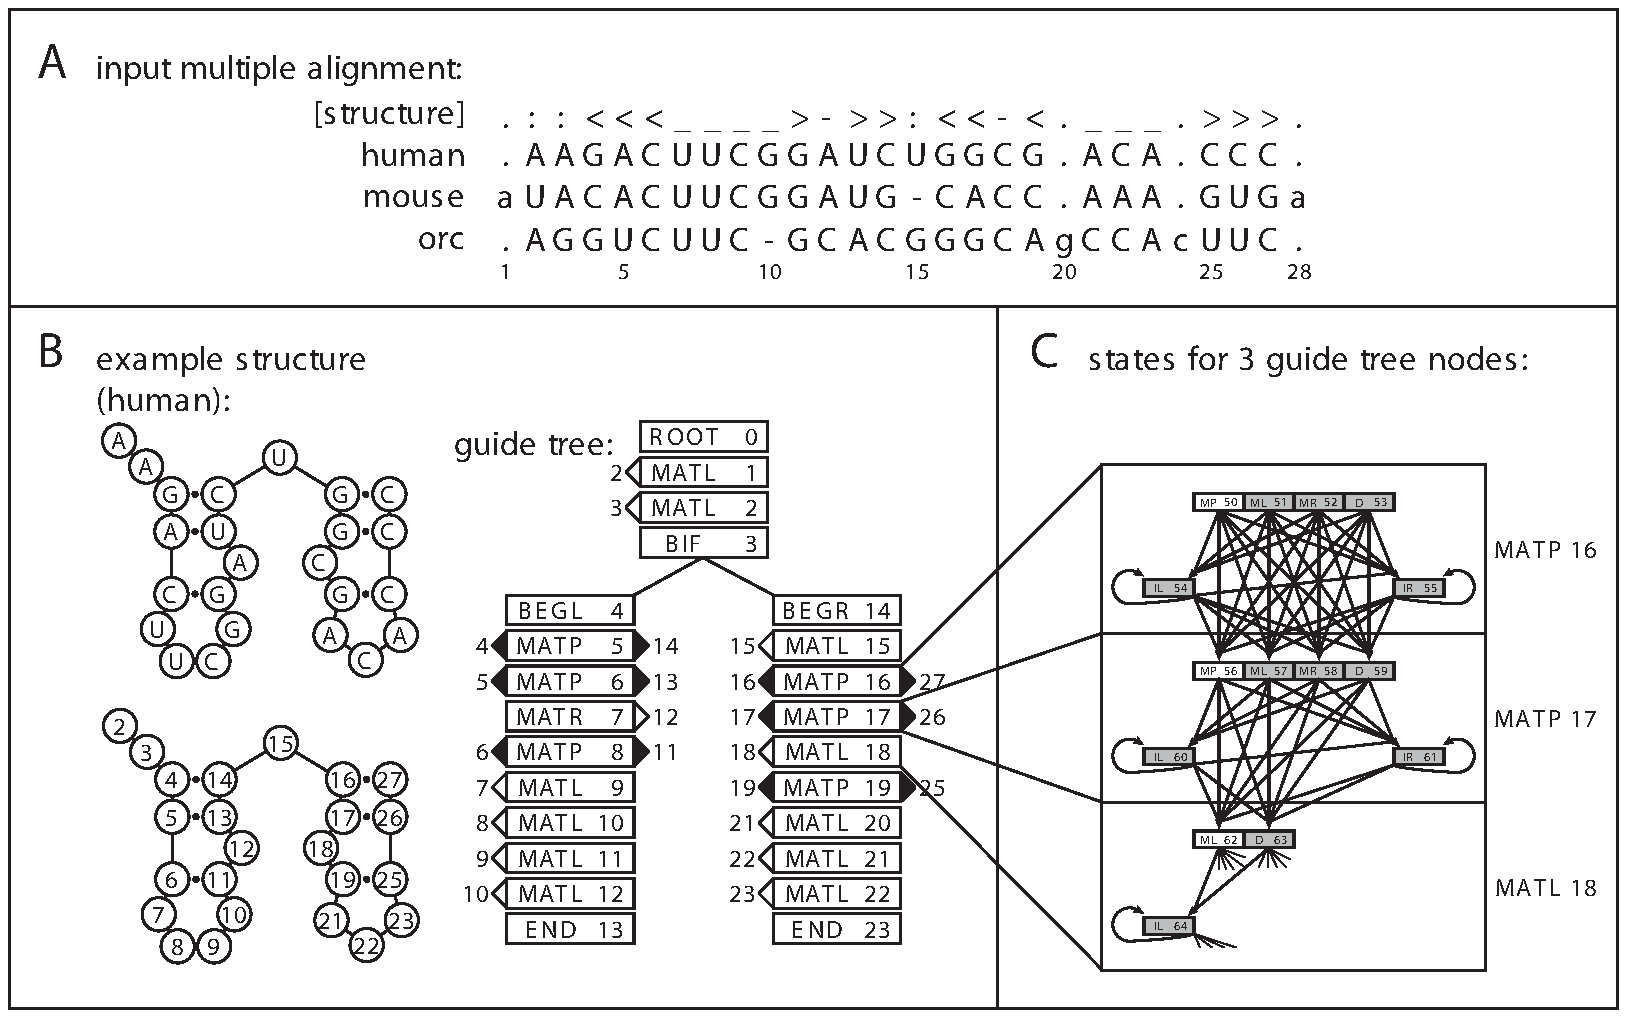
\includegraphics[width=6.4in]{figs/cmintro_bandcyk}
\caption{\textbf{An example RNA family and corresponding CM.}
  \textbf{(A):} A toy multiple alignment of three RNA
  sequences. \textbf{(B):} The structure of one sequence from (A), the
  same structure with positions numbered according to alignment
  columns, and the guide tree of nodes corresponding to that
  structure, with alignment column indices assigned to nodes (for
  example, node 5, a MATP ``match-pair'' node, will model the
  consensus base pair between columns 4 and 14). \textbf{(C):} The
  state topology of three selected nodes of the CM, for two MATP nodes
  and one consensus ``leftwise'' single residue bulge node (MATL,
  ``match-left'').  The consensus pair and singlet states (two MPs and
  one ML) are white, and the insertion/deletion states are grey. State
  transitions are indicated by arrows.}
\label{fig:cmintro}
\end{center}
\end{figure}


\newpage
\begin{figure}
  \begin{center}
    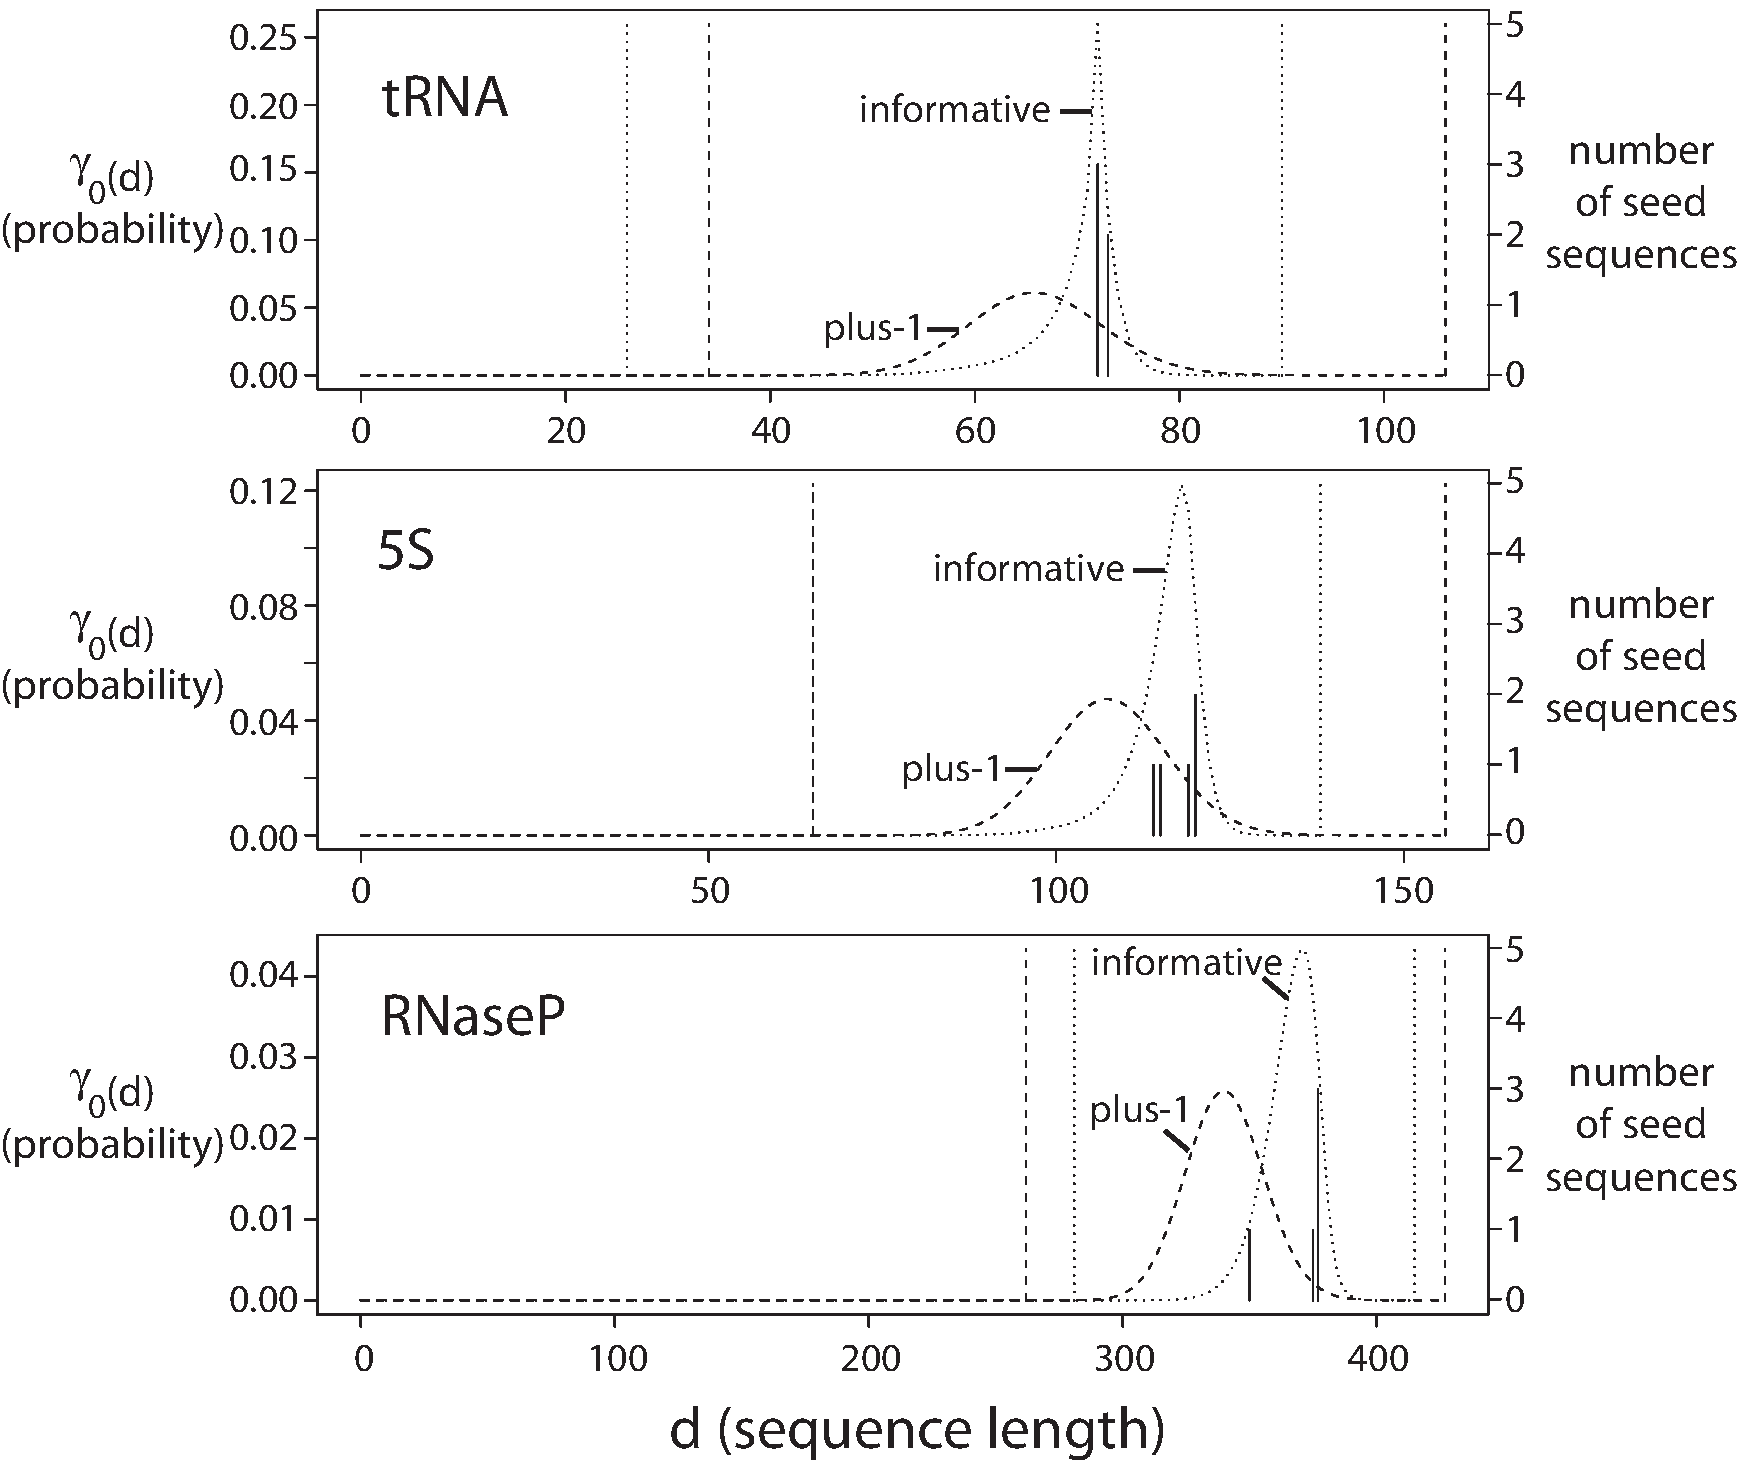
\includegraphics[width=6in,angle=0]{figs/3fam_bands}
    \caption{\textbf{Effect of transition priors on band calculation.}
      Predicted and actual target lengths are shown for three CMs
      built from alignments of five tRNA, 5S rRNA, and RNaseP
      sequences, which are about 75, 120, and 380 residues long,
      respectively.  Solid vertical lines represent the actual lengths
      of the sequences in each alignment, corresponding with the right
      vertical axis labels. Dashed and dotted curves show QDB
      calculations for $\gamma_0(d)$ for the root state of each model,
      for uninformative versus informative Dirichlet priors,
      respectively.  Dashed and dotted vertical lines show the band
      bounds ($d_{\mbox{min}}(0)$ (left) and $d_{\mbox{max}}(0)$
      (right)) derived from the $\gamma_0(d)$ distributions using
      $\beta = 10^{-7}$. The uninformative plus-one prior results in
      consistent underprediction of target sequence lengths, with a
      broad distribution. The new informative priors produce tighter
      distributions that are centered on the actual subsequence
      lengths. We observe the same result for all other states
      (data not shown).}
    \label{fig:bands}
  \end{center}
\end{figure}


\newpage
\begin{figure}
\begin{center}
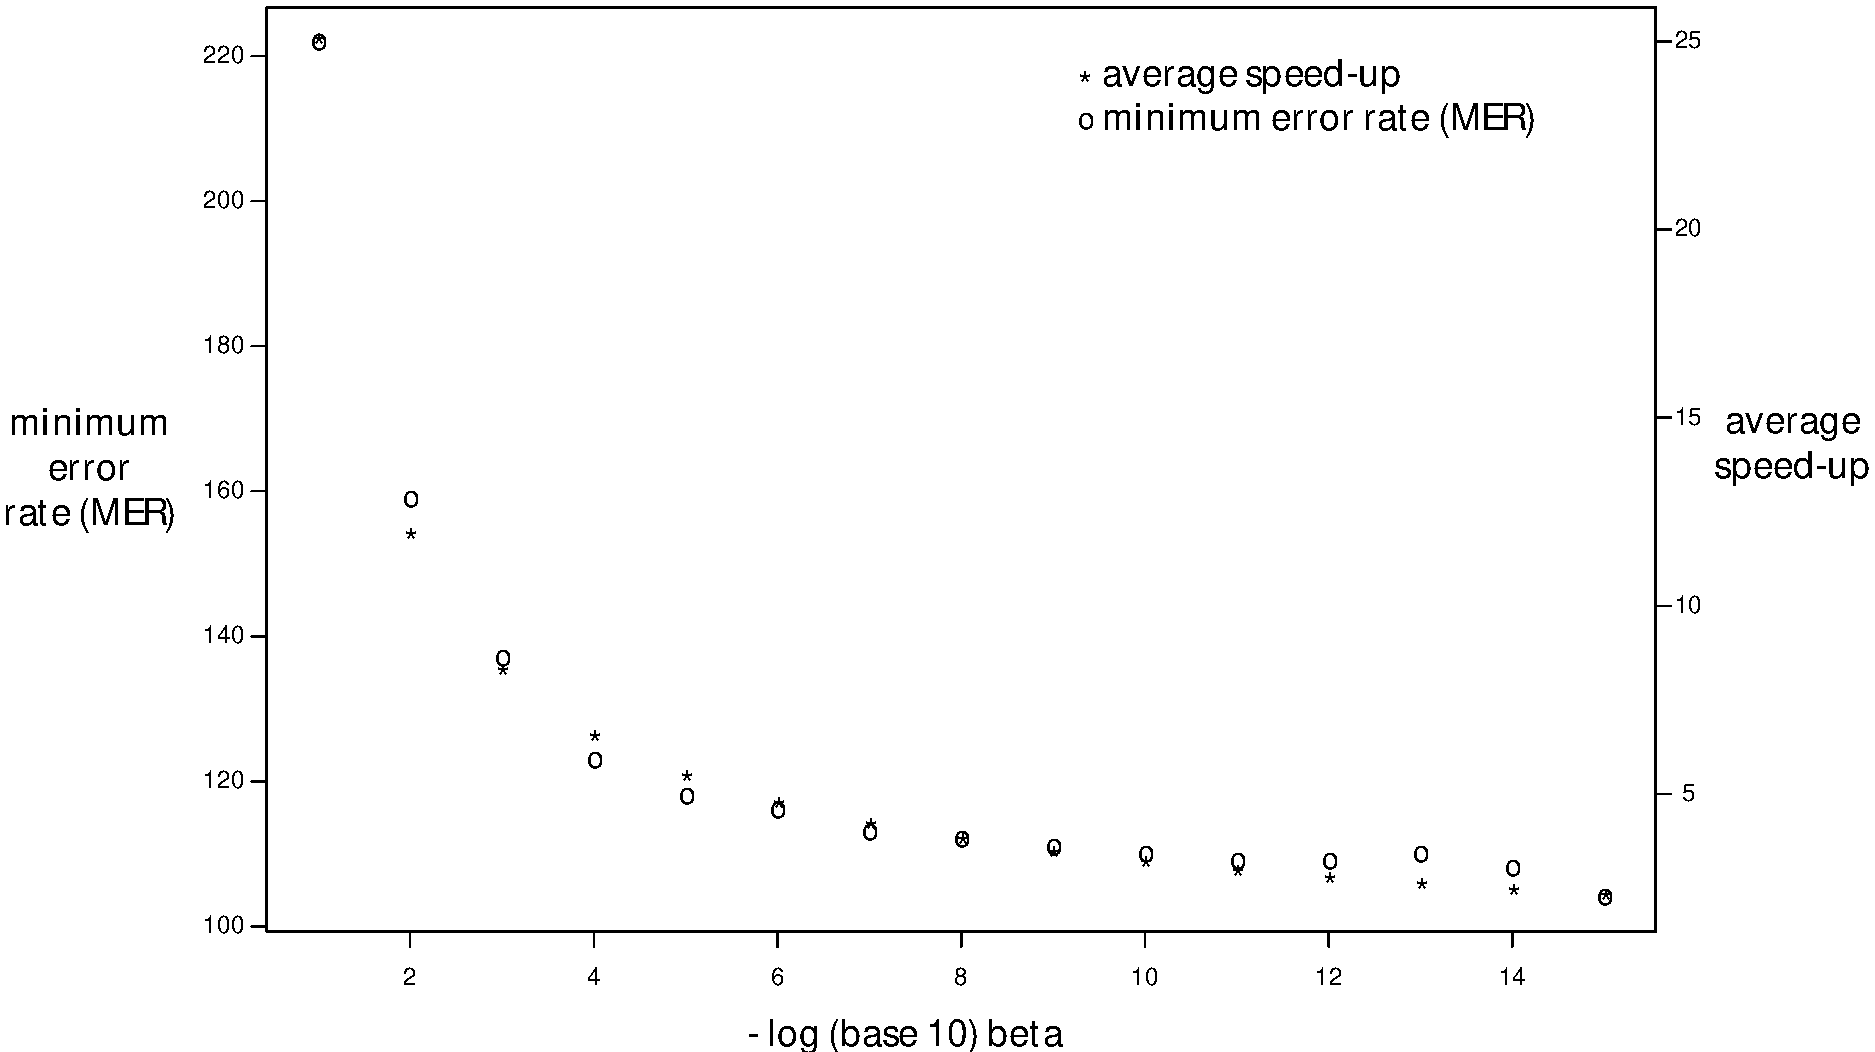
\includegraphics[width=6.4in]{figs/d5_beta_vs}
\caption{\textbf{Effect of varying the $\beta$ parameter on
    sensitivity, specificity, and speedup.}
}
\label{fig:betavaried}
\end{center}
\end{figure}


\newpage
\begin{figure}
\begin{center}
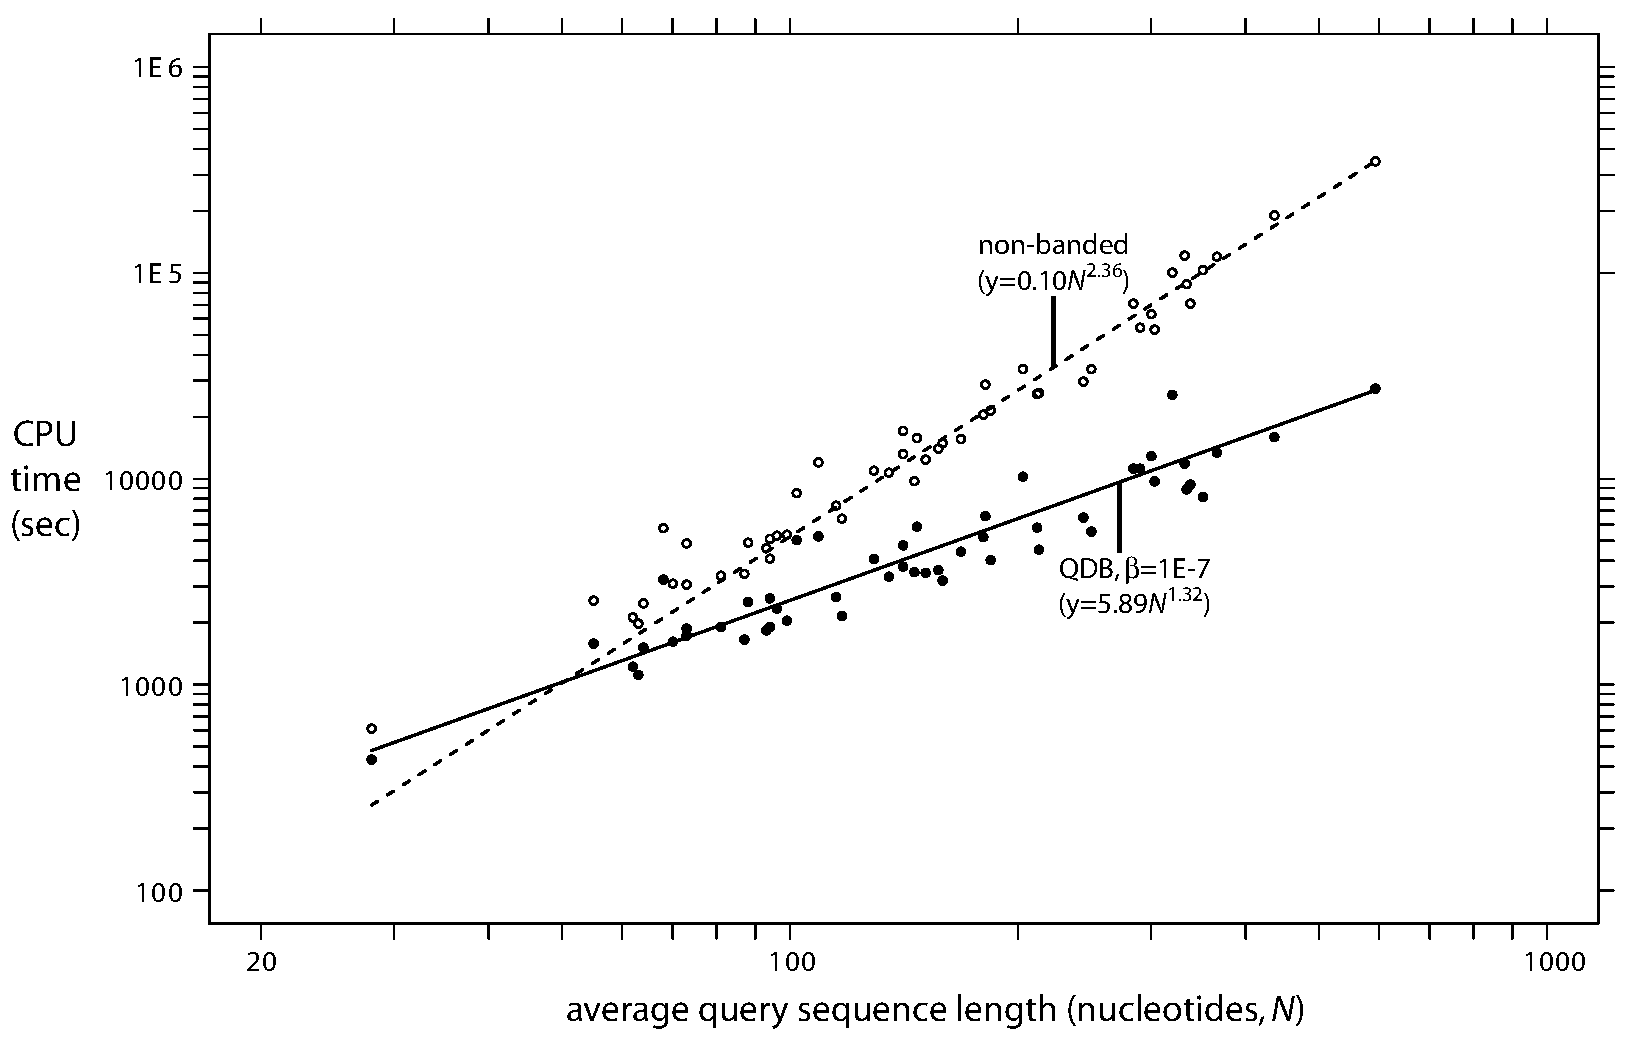
\includegraphics[width=6.4in]{figs/speedup}
\caption{\textbf{CPU time required by CM searches with and without
    QDB.} The time required for searching the 1 Mb target pseudogenome
    with each of the 51 benchmark models is shown as a point, plotted
    on a log-log graph as a function of the average length of the RNA
    sequences in the query alignment; open circles are without QDB,
    and filled circles are with QDB (with the default $\beta =
    1e-7$). Lines represent fits to a power law ($aN^b$), showing that
    for a fixed $L=$ 1 Mb target database size, the standard CYK
    algorithm empirically scales as $N^{2.36}$ and the QDB algorithm
    scales as $N^{1.32}$. The apparent intersection of the linear
    fitted lines is deceptive. At small query lengths,
    run time is dominated by factors other than the CM alignment
    computation, such as i/o. QDB searches are always faster
    than non-banded searches even for synthetic tiny
    queries of less than 10 nt (data not shown).}
\label{fig:speedup}
\end{center}
\end{figure}




\newpage
\begin{figure}
\begin{center}
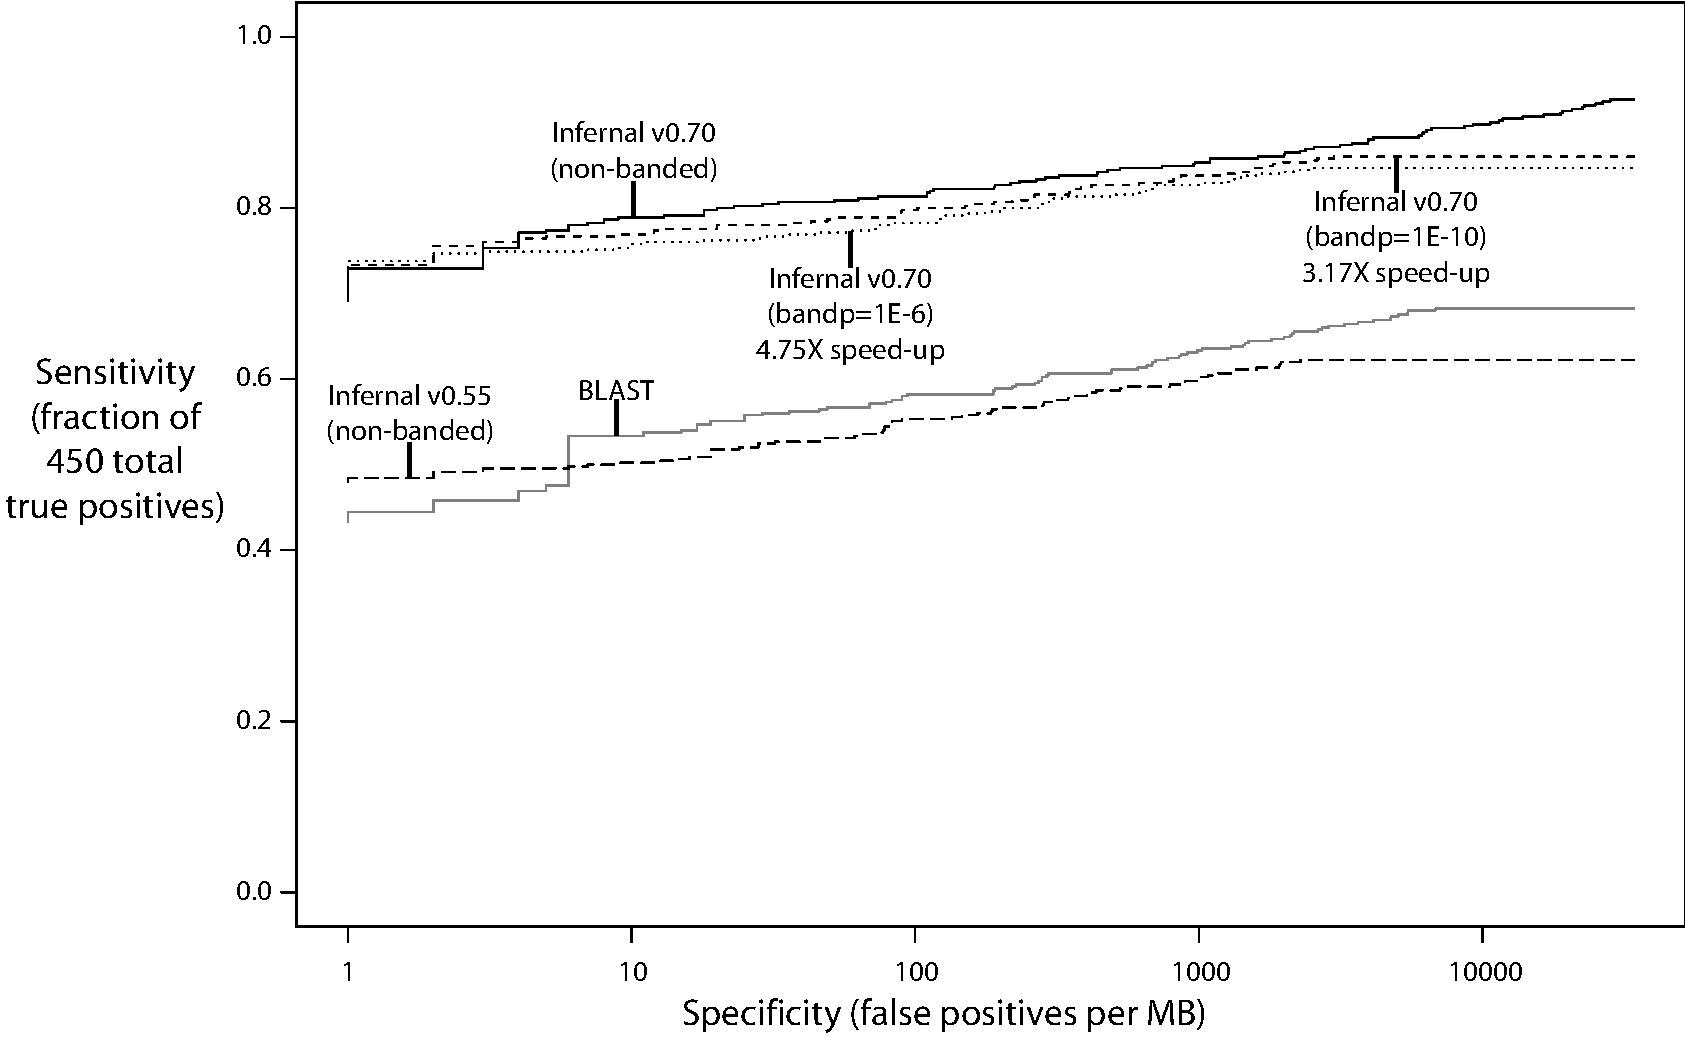
\includegraphics[width=6.4in,angle=0]{figs/d2roc_ai}
\end{center}
\caption{\textbf{ROC curves for the benchmark.}  Plots are shown for
the new \textsc{Infernal} 0.71 with and without QDB, for the old
\textsc{Infernal 0.55}, and for family-pairwise-searches with BLASTN.
}
\label{fig:roc}
\end{figure}

\fi

\end{document}
